\documentclass[11pt]{article}
\usepackage[utf8]{inputenc}
\usepackage[T1]{fontenc}
\usepackage{textcomp}
\usepackage[a4paper,margin=2.1cm]{geometry}
\usepackage{amsmath,amssymb}
\usepackage{graphicx}
\usepackage{tikz}
\usetikzlibrary{positioning,arrows.meta}
\usepackage{xcolor}
\usepackage{mdframed}
\usepackage[colorlinks=true,linkcolor=blue!60!black]{hyperref}
\setlength{\parindent}{0pt}
\setlength{\parskip}{6pt}

\newcommand{\question}[1]{\par\medskip\noindent\textbf{#1}\par}
\newmdenv[linecolor=green!45!black,linewidth=0.8pt,backgroundcolor=green!4,
  innertopmargin=4pt,innerbottommargin=4pt,skipabove=6pt,skipbelow=6pt]{answerbox}

\title{\textbf{Laws of Indices}\\[0.3em]\large Worked Solutions with TikZ Diagrams}
\author{Wisest Maths --- Year 1 A-Level, Algebra (ref \texttt{a4})}
\date{}

\begin{document}
\maketitle
\noindent This document contains all 50 \emph{Laws of Indices} questions, each with a fully
worked solution and a TikZ diagram matched to the law in play:
\begin{itemize}\setlength{\itemsep}{1pt}
  \item \textbf{Law cards} --- the boxed general rule with the exponent arithmetic --- for the multiplication, division, power-of-a-power, power-of-a-product, negative-power and zero-power laws;
  \item \textbf{Power/root split} diagrams for fractional indices (denominator $=$ root, numerator $=$ power);
  \item \textbf{Solution-flow} diagrams (one law per arrow) for multi-step numeric chains and for solving $a^{x}=k$.
\end{itemize}
\tableofcontents
\bigskip
\hrule

\section*{Laws of Indices 01\quad\small\texttt{(a4-001)}}
\addcontentsline{toc}{section}{Laws of Indices 01 (a4-001)}
\textit{Difficulty: Foundation \quad\textbar\quad Marks: 1}

\question{Simplify, leaving your answer as a power: \( 5^3 \times 5^4 \)}

\textbf{Worked solution.}

\textit{Step 1: When multiplying powers with the same base, add the exponents.}
\[\begin{gathered}
5^3 \times 5^4 = 5^{3+4}
\end{gathered}\]
The multiplication law of indices says \( a^m \times a^n = a^{m+n} \).

\textit{Step 2: Add the exponents together.}
\[\begin{gathered}
5^{7}
\end{gathered}\]
\( 3 + 4 = 7 \).

\begin{answerbox}
\textbf{Final answer:}\quad \(\displaystyle 5^{7}\)
\end{answerbox}
\textbf{Diagram.}

\begin{center}
\resizebox{\ifdim\width>\linewidth \linewidth\else \width\fi}{!}{%
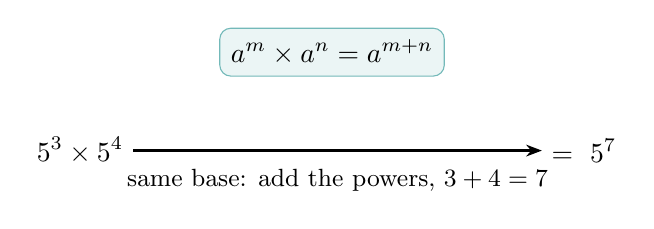
\begin{tikzpicture}[>={Stealth[length=2mm]}]
\node[draw=teal!55,rounded corners,fill=teal!8,inner sep=4pt] (rule) at (3.2,1.25) {$\displaystyle a^{m}\times a^{n}=a^{m+n}$};
\node (L) at (0,0) {$\displaystyle 5^{3}\times 5^{4}$};
\node (R) at (6.4,0) {$\displaystyle =\ 5^{7}$};
\draw[->,thick] (L) -- (R) node[midway,below=3pt,font=\small,align=center]{same base: add the powers, $3+4=7$};
\end{tikzpicture}
}
\end{center}
\small Index-law card: the boxed general rule (teal) is applied to the expression.\normalsize

\medskip\hrule

\section*{Laws of Indices 02\quad\small\texttt{(a4-002)}}
\addcontentsline{toc}{section}{Laws of Indices 02 (a4-002)}
\textit{Difficulty: Foundation \quad\textbar\quad Marks: 1}

\question{Simplify, leaving your answer as a power: \( 8^5 \div 8^2 \)}

\textbf{Worked solution.}

\textit{Step 1: When dividing powers with the same base, subtract the exponents.}
\[\begin{gathered}
8^5 \div 8^2 = 8^{5-2}
\end{gathered}\]
The division law of indices says \( a^m \div a^n = a^{m-n} \).

\textit{Step 2: Subtract the exponents.}
\[\begin{gathered}
8^{3}
\end{gathered}\]
\( 5 - 2 = 3 \).

\begin{answerbox}
\textbf{Final answer:}\quad \(\displaystyle 8^{3}\)
\end{answerbox}
\textbf{Diagram.}

\begin{center}
\resizebox{\ifdim\width>\linewidth \linewidth\else \width\fi}{!}{%
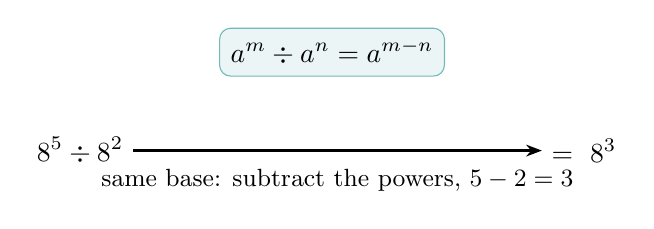
\begin{tikzpicture}[>={Stealth[length=2mm]}]
\node[draw=teal!55,rounded corners,fill=teal!8,inner sep=4pt] (rule) at (3.2,1.25) {$\displaystyle a^{m}\div a^{n}=a^{m-n}$};
\node (L) at (0,0) {$\displaystyle 8^{5}\div 8^{2}$};
\node (R) at (6.4,0) {$\displaystyle =\ 8^{3}$};
\draw[->,thick] (L) -- (R) node[midway,below=3pt,font=\small,align=center]{same base: subtract the powers, $5-2=3$};
\end{tikzpicture}
}
\end{center}
\small Index-law card: the boxed general rule (teal) is applied to the expression.\normalsize

\medskip\hrule

\section*{Laws of Indices 03\quad\small\texttt{(a4-003)}}
\addcontentsline{toc}{section}{Laws of Indices 03 (a4-003)}
\textit{Difficulty: Foundation \quad\textbar\quad Marks: 1}

\question{Simplify, leaving your answer as a power: \( (6^3)^2 \)}

\textbf{Worked solution.}

\textit{Step 1: When raising a power to another power, multiply the exponents.}
\[\begin{gathered}
(6^3)^2 = 6^{3 \times 2}
\end{gathered}\]
The power-of-a-power law says \( (a^m)^n = a^{mn} \).

\textit{Step 2: Multiply the exponents together.}
\[\begin{gathered}
6^{6}
\end{gathered}\]
\( 3 \times 2 = 6 \).

\begin{answerbox}
\textbf{Final answer:}\quad \(\displaystyle 6^{6}\)
\end{answerbox}
\textbf{Diagram.}

\begin{center}
\resizebox{\ifdim\width>\linewidth \linewidth\else \width\fi}{!}{%
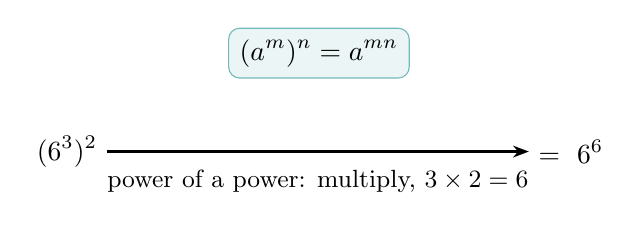
\begin{tikzpicture}[>={Stealth[length=2mm]}]
\node[draw=teal!55,rounded corners,fill=teal!8,inner sep=4pt] (rule) at (3.2,1.25) {$\displaystyle (a^{m})^{n}=a^{mn}$};
\node (L) at (0,0) {$\displaystyle (6^{3})^{2}$};
\node (R) at (6.4,0) {$\displaystyle =\ 6^{6}$};
\draw[->,thick] (L) -- (R) node[midway,below=3pt,font=\small,align=center]{power of a power: multiply, $3\times 2=6$};
\end{tikzpicture}
}
\end{center}
\small Index-law card: the boxed general rule (teal) is applied to the expression.\normalsize

\medskip\hrule

\section*{Laws of Indices 04\quad\small\texttt{(a4-004)}}
\addcontentsline{toc}{section}{Laws of Indices 04 (a4-004)}
\textit{Difficulty: Foundation \quad\textbar\quad Marks: 2}

\question{Simplify, leaving your answer as a single power of \( y \): \( y^{-1} \times y^2 \times y^3 \)}

\textbf{Worked solution.}

\textit{Step 1: Add all the exponents together since the bases are the same and the terms are multiplied.}
\[\begin{gathered}
y^{-1+2+3}
\end{gathered}\]
The multiplication law applies to any number of terms: \( a^m \times a^n \times a^p = a^{m+n+p} \).

\textit{Step 2: Simplify the sum of the exponents.}
\[\begin{gathered}
y^{4}
\end{gathered}\]
\( -1 + 2 + 3 = 4 \).

\begin{answerbox}
\textbf{Final answer:}\quad \(\displaystyle y^{4}\)
\end{answerbox}
\textbf{Diagram.}

\begin{center}
\resizebox{\ifdim\width>\linewidth \linewidth\else \width\fi}{!}{%
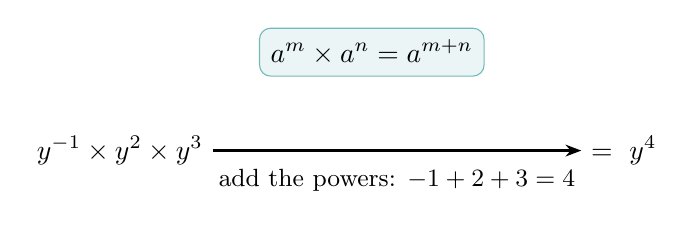
\begin{tikzpicture}[>={Stealth[length=2mm]}]
\node[draw=teal!55,rounded corners,fill=teal!8,inner sep=4pt] (rule) at (3.2,1.25) {$\displaystyle a^{m}\times a^{n}=a^{m+n}$};
\node (L) at (0,0) {$\displaystyle y^{-1}\times y^{2}\times y^{3}$};
\node (R) at (6.4,0) {$\displaystyle =\ y^{4}$};
\draw[->,thick] (L) -- (R) node[midway,below=3pt,font=\small,align=center]{add the powers: $-1+2+3=4$};
\end{tikzpicture}
}
\end{center}
\small Index-law card: the boxed general rule (teal) is applied to the expression.\normalsize

\medskip\hrule

\section*{Laws of Indices 05\quad\small\texttt{(a4-005)}}
\addcontentsline{toc}{section}{Laws of Indices 05 (a4-005)}
\textit{Difficulty: Foundation \quad\textbar\quad Marks: 1}

\question{Simplify, leaving your answer as a power: \( \frac{6^{11}}{6^6} \)}

\textbf{Worked solution.}

\textit{Step 1: Writing the fraction as a division and subtracting exponents.}
\[\begin{gathered}
\frac{6^{11}}{6^6} = 6^{11-6}
\end{gathered}\]
A fraction with the same base on top and bottom is the same as dividing, so subtract the exponents.

\textit{Step 2: Simplify the exponent.}
\[\begin{gathered}
6^{5}
\end{gathered}\]
\( 11 - 6 = 5 \).

\begin{answerbox}
\textbf{Final answer:}\quad \(\displaystyle 6^{5}\)
\end{answerbox}
\textbf{Diagram.}

\begin{center}
\resizebox{\ifdim\width>\linewidth \linewidth\else \width\fi}{!}{%
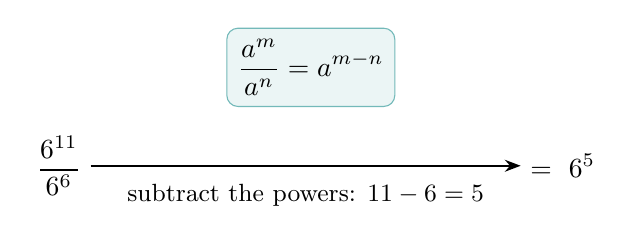
\begin{tikzpicture}[>={Stealth[length=2mm]}]
\node[draw=teal!55,rounded corners,fill=teal!8,inner sep=4pt] (rule) at (3.2,1.25) {$\displaystyle \dfrac{a^{m}}{a^{n}}=a^{m-n}$};
\node (L) at (0,0) {$\displaystyle \dfrac{6^{11}}{6^{6}}$};
\node (R) at (6.4,0) {$\displaystyle =\ 6^{5}$};
\draw[->,thick] (L) -- (R) node[midway,below=3pt,font=\small,align=center]{subtract the powers: $11-6=5$};
\end{tikzpicture}
}
\end{center}
\small Index-law card: the boxed general rule (teal) is applied to the expression.\normalsize

\medskip\hrule

\section*{Laws of Indices 06\quad\small\texttt{(a4-006)}}
\addcontentsline{toc}{section}{Laws of Indices 06 (a4-006)}
\textit{Difficulty: Foundation \quad\textbar\quad Marks: 1}

\question{Simplify, leaving your answer as a single power of \( r \): \( \frac{r^2}{r^6} \)}

\textbf{Worked solution.}

\textit{Step 1: Subtract the exponents using the division law.}
\[\begin{gathered}
r^{2-6}
\end{gathered}\]
Subtract the bottom exponent from the top exponent.

\textit{Step 2: Simplify the exponent.}
\[\begin{gathered}
r^{-4}
\end{gathered}\]
\( 2 - 6 = -4 \). A negative exponent is perfectly valid here.

\begin{answerbox}
\textbf{Final answer:}\quad \(\displaystyle r^{-4}\)
\end{answerbox}
\textbf{Diagram.}

\begin{center}
\resizebox{\ifdim\width>\linewidth \linewidth\else \width\fi}{!}{%
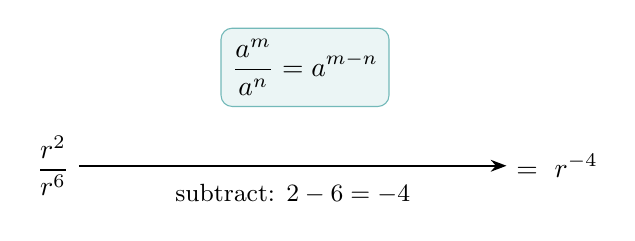
\begin{tikzpicture}[>={Stealth[length=2mm]}]
\node[draw=teal!55,rounded corners,fill=teal!8,inner sep=4pt] (rule) at (3.2,1.25) {$\displaystyle \dfrac{a^{m}}{a^{n}}=a^{m-n}$};
\node (L) at (0,0) {$\displaystyle \dfrac{r^{2}}{r^{6}}$};
\node (R) at (6.4,0) {$\displaystyle =\ r^{-4}$};
\draw[->,thick] (L) -- (R) node[midway,below=3pt,font=\small,align=center]{subtract: $2-6=-4$};
\end{tikzpicture}
}
\end{center}
\small Index-law card: the boxed general rule (teal) is applied to the expression.\normalsize

\medskip\hrule

\section*{Laws of Indices 07\quad\small\texttt{(a4-007)}}
\addcontentsline{toc}{section}{Laws of Indices 07 (a4-007)}
\textit{Difficulty: Foundation \quad\textbar\quad Marks: 1}

\question{Simplify: \( (k^{-2})^5 \)}

\textbf{Worked solution.}

\textit{Step 1: Multiply the exponents using the power-of-a-power law.}
\[\begin{gathered}
k^{-2 \times 5}
\end{gathered}\]
\( (a^m)^n = a^{mn} \), even when \( m \) is negative.

\textit{Step 2: Evaluate the product of the exponents.}
\[\begin{gathered}
k^{-10}
\end{gathered}\]
\( -2 \times 5 = -10 \).

\begin{answerbox}
\textbf{Final answer:}\quad \(\displaystyle k^{-10}\)
\end{answerbox}
\textbf{Diagram.}

\begin{center}
\resizebox{\ifdim\width>\linewidth \linewidth\else \width\fi}{!}{%
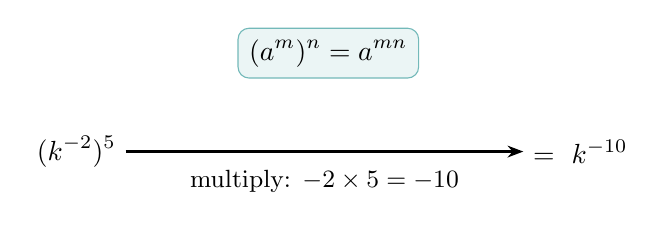
\begin{tikzpicture}[>={Stealth[length=2mm]}]
\node[draw=teal!55,rounded corners,fill=teal!8,inner sep=4pt] (rule) at (3.2,1.25) {$\displaystyle (a^{m})^{n}=a^{mn}$};
\node (L) at (0,0) {$\displaystyle (k^{-2})^{5}$};
\node (R) at (6.4,0) {$\displaystyle =\ k^{-10}$};
\draw[->,thick] (L) -- (R) node[midway,below=3pt,font=\small,align=center]{multiply: $-2\times 5=-10$};
\end{tikzpicture}
}
\end{center}
\small Index-law card: the boxed general rule (teal) is applied to the expression.\normalsize

\medskip\hrule

\section*{Laws of Indices 08\quad\small\texttt{(a4-008)}}
\addcontentsline{toc}{section}{Laws of Indices 08 (a4-008)}
\textit{Difficulty: Foundation \quad\textbar\quad Marks: 2}

\question{Evaluate: \( 4^{\frac{1}{2}} \times 4^{\frac{1}{2}} \)}

\textbf{Worked solution.}

\textit{Step 1: Add the fractional exponents since the bases are the same.}
\[\begin{gathered}
4^{\frac{1}{2}+\frac{1}{2}} = 4^{1}
\end{gathered}\]
\( \frac{1}{2} + \frac{1}{2} = 1 \).

\textit{Step 2: Evaluate.}
\[\begin{gathered}
4
\end{gathered}\]
Any number to the power 1 is itself.

\begin{answerbox}
\textbf{Final answer:}\quad \(\displaystyle 4\)
\end{answerbox}
\textbf{Diagram.}

\begin{center}
\resizebox{\ifdim\width>\linewidth \linewidth\else \width\fi}{!}{%
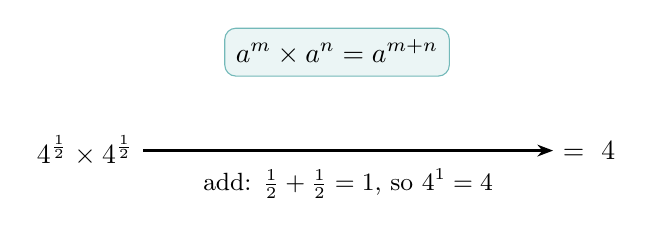
\begin{tikzpicture}[>={Stealth[length=2mm]}]
\node[draw=teal!55,rounded corners,fill=teal!8,inner sep=4pt] (rule) at (3.2,1.25) {$\displaystyle a^{m}\times a^{n}=a^{m+n}$};
\node (L) at (0,0) {$\displaystyle 4^{\frac{1}{2}}\times 4^{\frac{1}{2}}$};
\node (R) at (6.4,0) {$\displaystyle =\ 4$};
\draw[->,thick] (L) -- (R) node[midway,below=3pt,font=\small,align=center]{add: $\tfrac12+\tfrac12=1$, so $4^{1}=4$};
\end{tikzpicture}
}
\end{center}
\small Index-law card: the boxed general rule (teal) is applied to the expression.\normalsize

\medskip\hrule

\section*{Laws of Indices 09\quad\small\texttt{(a4-009)}}
\addcontentsline{toc}{section}{Laws of Indices 09 (a4-009)}
\textit{Difficulty: Foundation \quad\textbar\quad Marks: 2}

\question{Evaluate: \( 3^4 \div 3^1 \)}

\textbf{Worked solution.}

\textit{Step 1: Subtract the exponents using the division law.}
\[\begin{gathered}
3^{4-1} = 3^{3}
\end{gathered}\]
\( a^m \div a^n = a^{m-n} \).

\textit{Step 2: Evaluate \( 3^3 \).}
\[\begin{gathered}
3 \times 3 \times 3 = 27
\end{gathered}\]
Multiply three copies of 3 together.

\begin{answerbox}
\textbf{Final answer:}\quad \(\displaystyle 27\)
\end{answerbox}
\textbf{Diagram.}

\begin{center}
\resizebox{\ifdim\width>\linewidth \linewidth\else \width\fi}{!}{%
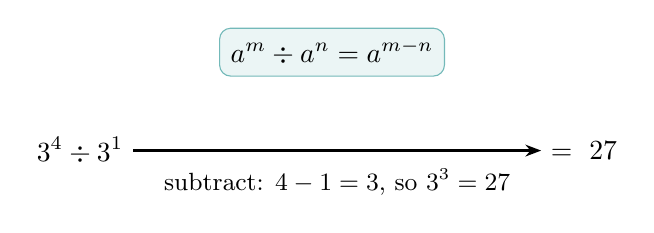
\begin{tikzpicture}[>={Stealth[length=2mm]}]
\node[draw=teal!55,rounded corners,fill=teal!8,inner sep=4pt] (rule) at (3.2,1.25) {$\displaystyle a^{m}\div a^{n}=a^{m-n}$};
\node (L) at (0,0) {$\displaystyle 3^{4}\div 3^{1}$};
\node (R) at (6.4,0) {$\displaystyle =\ 27$};
\draw[->,thick] (L) -- (R) node[midway,below=3pt,font=\small,align=center]{subtract: $4-1=3$, so $3^{3}=27$};
\end{tikzpicture}
}
\end{center}
\small Index-law card: the boxed general rule (teal) is applied to the expression.\normalsize

\medskip\hrule

\section*{Laws of Indices 10\quad\small\texttt{(a4-010)}}
\addcontentsline{toc}{section}{Laws of Indices 10 (a4-010)}
\textit{Difficulty: Foundation \quad\textbar\quad Marks: 2}

\question{Evaluate: \( (2^3)^2 \div 2^4 \)}

\textbf{Worked solution.}

\textit{Step 1: Apply the power-of-a-power law to simplify \( (2^3)^2 \).}
\[\begin{gathered}
2^{3 \times 2} \div 2^4 = 2^6 \div 2^4
\end{gathered}\]
Multiply the exponents inside the bracket first.

\textit{Step 2: Now apply the division law.}
\[\begin{gathered}
2^{6-4} = 2^2
\end{gathered}\]
Subtract the exponents since the bases are the same.

\textit{Step 3: Evaluate \( 2^2 \).}
\[\begin{gathered}
4
\end{gathered}\]
\( 2 \times 2 = 4 \).

\begin{answerbox}
\textbf{Final answer:}\quad \(\displaystyle 4\)
\end{answerbox}
\textbf{Diagram.}

\begin{center}
\resizebox{\ifdim\width>\linewidth \linewidth\else \width\fi}{!}{%
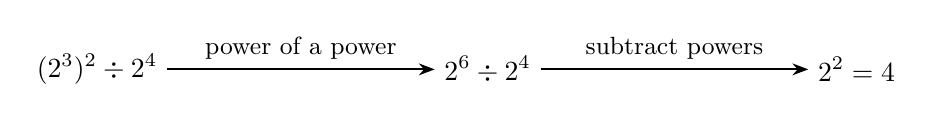
\begin{tikzpicture}[>={Stealth[length=2mm]},node distance=1.5cm and 3.4cm]
\node (s0) {$\displaystyle (2^{3})^{2}\div 2^{4}$};
\node (s1) [right=of s0] {$\displaystyle 2^{6}\div 2^{4}$};
\node (s2) [right=of s1] {$\displaystyle 2^{2}=4$};
\draw[->,thick] (s0) -- (s1) node[midway,above,font=\small]{power of a power};
\draw[->,thick] (s1) -- (s2) node[midway,above,font=\small]{subtract powers};
\end{tikzpicture}
}
\end{center}
\small Solution flow: each arrow applies one index law.\normalsize

\medskip\hrule

\section*{Laws of Indices 11\quad\small\texttt{(a4-011)}}
\addcontentsline{toc}{section}{Laws of Indices 11 (a4-011)}
\textit{Difficulty: Foundation \quad\textbar\quad Marks: 1}

\question{Evaluate: \( 7^0 \)}

\textbf{Worked solution.}

\textit{Apply the zero exponent rule.}
\[\begin{gathered}
7^0 = 1
\end{gathered}\]
Any non-zero number raised to the power 0 equals 1. This follows from the division law: \( a^n \div a^n = a^{n-n} = a^0 = 1 \).

\begin{answerbox}
\textbf{Final answer:}\quad \(\displaystyle 1\)
\end{answerbox}
\textbf{Diagram.}

\begin{center}
\resizebox{\ifdim\width>\linewidth \linewidth\else \width\fi}{!}{%
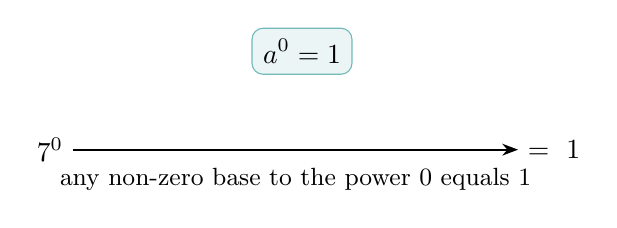
\begin{tikzpicture}[>={Stealth[length=2mm]}]
\node[draw=teal!55,rounded corners,fill=teal!8,inner sep=4pt] (rule) at (3.2,1.25) {$\displaystyle a^{0}=1$};
\node (L) at (0,0) {$\displaystyle 7^{0}$};
\node (R) at (6.4,0) {$\displaystyle =\ 1$};
\draw[->,thick] (L) -- (R) node[midway,below=3pt,font=\small,align=center]{any non-zero base to the power $0$ equals $1$};
\end{tikzpicture}
}
\end{center}
\small Index-law card: the boxed general rule (teal) is applied to the expression.\normalsize

\medskip\hrule

\section*{Laws of Indices 12\quad\small\texttt{(a4-012)}}
\addcontentsline{toc}{section}{Laws of Indices 12 (a4-012)}
\textit{Difficulty: Foundation \quad\textbar\quad Marks: 1}

\question{Evaluate: \( \left(\frac{3}{5}\right)^0 \)}

\textbf{Worked solution.}

\textit{Apply the zero exponent rule.}
\[\begin{gathered}
\left(\frac{3}{5}\right)^0 = 1
\end{gathered}\]
Anything (except zero) raised to the power 0 is 1 — it does not matter whether it is a whole number or a fraction.

\begin{answerbox}
\textbf{Final answer:}\quad \(\displaystyle 1\)
\end{answerbox}
\textbf{Diagram.}

\begin{center}
\resizebox{\ifdim\width>\linewidth \linewidth\else \width\fi}{!}{%
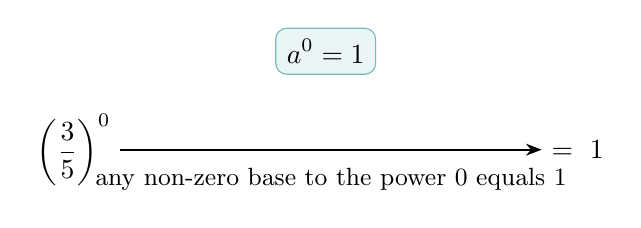
\begin{tikzpicture}[>={Stealth[length=2mm]}]
\node[draw=teal!55,rounded corners,fill=teal!8,inner sep=4pt] (rule) at (3.2,1.25) {$\displaystyle a^{0}=1$};
\node (L) at (0,0) {$\displaystyle \left(\dfrac{3}{5}\right)^{0}$};
\node (R) at (6.4,0) {$\displaystyle =\ 1$};
\draw[->,thick] (L) -- (R) node[midway,below=3pt,font=\small,align=center]{any non-zero base to the power $0$ equals $1$};
\end{tikzpicture}
}
\end{center}
\small Index-law card: the boxed general rule (teal) is applied to the expression.\normalsize

\medskip\hrule

\section*{Laws of Indices 13\quad\small\texttt{(a4-013)}}
\addcontentsline{toc}{section}{Laws of Indices 13 (a4-013)}
\textit{Difficulty: Foundation \quad\textbar\quad Marks: 1}

\question{Evaluate: \( 9^{\frac{1}{2}} \)}

\textbf{Worked solution.}

\textit{Step 1: Recognise that a power of \( \frac{1}{2} \) means the square root.}
\[\begin{gathered}
9^{\frac{1}{2}} = \sqrt{9}
\end{gathered}\]
\( a^{\frac{1}{2}} = \sqrt{a} \).

\textit{Step 2: Evaluate the square root.}
\[\begin{gathered}
3
\end{gathered}\]
\( 3 \times 3 = 9 \), so \( \sqrt{9} = 3 \).

\begin{answerbox}
\textbf{Final answer:}\quad \(\displaystyle 3\)
\end{answerbox}
\textbf{Diagram.}

\begin{center}
\resizebox{\ifdim\width>\linewidth \linewidth\else \width\fi}{!}{%
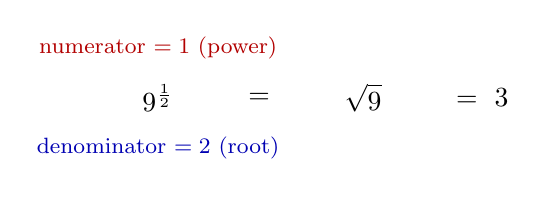
\begin{tikzpicture}[node distance=5mm and 7mm]
\node (e) {$\displaystyle 9^{\frac{1}{2}}$};
\node (eq) [right=of e] {$=$};
\node (mid) [right=of eq] {$\displaystyle \sqrt{9}$};
\node (res) [right=of mid] {$\displaystyle =\ 3$};
\node[red!70!black,font=\footnotesize,above=2pt of e] {numerator $=1$ (power)};
\node[blue!70!black,font=\footnotesize,below=2pt of e] {denominator $=2$ (root)};
\end{tikzpicture}
}
\end{center}
\small Fractional index: the \emph{denominator} gives the root, the \emph{numerator} gives the power.\normalsize

\medskip\hrule

\section*{Laws of Indices 14\quad\small\texttt{(a4-014)}}
\addcontentsline{toc}{section}{Laws of Indices 14 (a4-014)}
\textit{Difficulty: Foundation \quad\textbar\quad Marks: 1}

\question{Evaluate: \( 8^{\frac{1}{3}} \)}

\textbf{Worked solution.}

\textit{Step 1: Recognise that a power of \( \frac{1}{3} \) means the cube root.}
\[\begin{gathered}
8^{\frac{1}{3}} = \sqrt[3]{8}
\end{gathered}\]
\( a^{\frac{1}{3}} = \sqrt[3]{a} \).

\textit{Step 2: Evaluate the cube root.}
\[\begin{gathered}
2
\end{gathered}\]
\( 2 \times 2 \times 2 = 8 \), so the cube root of 8 is 2.

\begin{answerbox}
\textbf{Final answer:}\quad \(\displaystyle 2\)
\end{answerbox}
\textbf{Diagram.}

\begin{center}
\resizebox{\ifdim\width>\linewidth \linewidth\else \width\fi}{!}{%
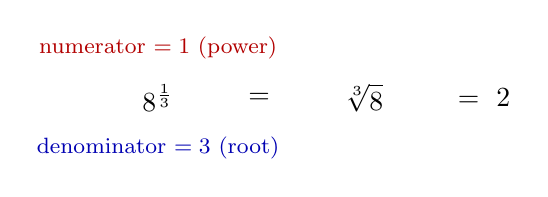
\begin{tikzpicture}[node distance=5mm and 7mm]
\node (e) {$\displaystyle 8^{\frac{1}{3}}$};
\node (eq) [right=of e] {$=$};
\node (mid) [right=of eq] {$\displaystyle \sqrt[3]{8}$};
\node (res) [right=of mid] {$\displaystyle =\ 2$};
\node[red!70!black,font=\footnotesize,above=2pt of e] {numerator $=1$ (power)};
\node[blue!70!black,font=\footnotesize,below=2pt of e] {denominator $=3$ (root)};
\end{tikzpicture}
}
\end{center}
\small Fractional index: the \emph{denominator} gives the root, the \emph{numerator} gives the power.\normalsize

\medskip\hrule

\section*{Laws of Indices 15\quad\small\texttt{(a4-015)}}
\addcontentsline{toc}{section}{Laws of Indices 15 (a4-015)}
\textit{Difficulty: Foundation \quad\textbar\quad Marks: 1}

\question{Evaluate: \( 27^{\frac{1}{3}} \)}

\textbf{Worked solution.}

\textit{Step 1: The exponent \( \frac{1}{3} \) means take the cube root.}
\[\begin{gathered}
27^{\frac{1}{3}} = \sqrt[3]{27}
\end{gathered}\]
Ask yourself: what number multiplied by itself three times gives 27?

\textit{Step 2: Evaluate.}
\[\begin{gathered}
3
\end{gathered}\]
\( 3 \times 3 \times 3 = 27 \).

\begin{answerbox}
\textbf{Final answer:}\quad \(\displaystyle 3\)
\end{answerbox}
\textbf{Diagram.}

\begin{center}
\resizebox{\ifdim\width>\linewidth \linewidth\else \width\fi}{!}{%
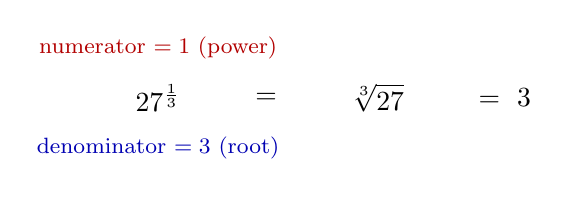
\begin{tikzpicture}[node distance=5mm and 7mm]
\node (e) {$\displaystyle 27^{\frac{1}{3}}$};
\node (eq) [right=of e] {$=$};
\node (mid) [right=of eq] {$\displaystyle \sqrt[3]{27}$};
\node (res) [right=of mid] {$\displaystyle =\ 3$};
\node[red!70!black,font=\footnotesize,above=2pt of e] {numerator $=1$ (power)};
\node[blue!70!black,font=\footnotesize,below=2pt of e] {denominator $=3$ (root)};
\end{tikzpicture}
}
\end{center}
\small Fractional index: the \emph{denominator} gives the root, the \emph{numerator} gives the power.\normalsize

\medskip\hrule

\section*{Laws of Indices 16\quad\small\texttt{(a4-016)}}
\addcontentsline{toc}{section}{Laws of Indices 16 (a4-016)}
\textit{Difficulty: Foundation \quad\textbar\quad Marks: 2}

\question{Evaluate: \( 16^{\frac{3}{4}} \)}

\textbf{Worked solution.}

\textit{Step 1: Split the fractional exponent: root first, then power.}
\[\begin{gathered}
16^{\frac{3}{4}} = \left(16^{\frac{1}{4}}\right)^3
\end{gathered}\]
The denominator 4 tells you to take the fourth root, and the numerator 3 tells you to cube the result.

\textit{Step 2: Evaluate the fourth root of 16.}
\[\begin{gathered}
16^{\frac{1}{4}} = 2
\end{gathered}\]
\( 2 \times 2 \times 2 \times 2 = 16 \).

\textit{Step 3: Cube the result.}
\[\begin{gathered}
2^3 = 8
\end{gathered}\]
\( 2 \times 2 \times 2 = 8 \).

\begin{answerbox}
\textbf{Final answer:}\quad \(\displaystyle 8\)
\end{answerbox}
\textbf{Diagram.}

\begin{center}
\resizebox{\ifdim\width>\linewidth \linewidth\else \width\fi}{!}{%
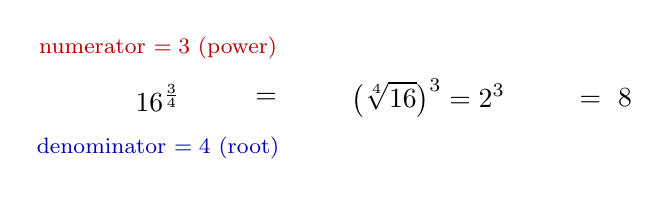
\begin{tikzpicture}[node distance=5mm and 7mm]
\node (e) {$\displaystyle 16^{\frac{3}{4}}$};
\node (eq) [right=of e] {$=$};
\node (mid) [right=of eq] {$\displaystyle \big(\sqrt[4]{16}\big)^{3}=2^{3}$};
\node (res) [right=of mid] {$\displaystyle =\ 8$};
\node[red!70!black,font=\footnotesize,above=2pt of e] {numerator $=3$ (power)};
\node[blue!70!black,font=\footnotesize,below=2pt of e] {denominator $=4$ (root)};
\end{tikzpicture}
}
\end{center}
\small Fractional index: the \emph{denominator} gives the root, the \emph{numerator} gives the power.\normalsize

\medskip\hrule

\section*{Laws of Indices 17\quad\small\texttt{(a4-017)}}
\addcontentsline{toc}{section}{Laws of Indices 17 (a4-017)}
\textit{Difficulty: Foundation \quad\textbar\quad Marks: 2}

\question{Evaluate: \( 25^{\frac{3}{2}} \)}

\textbf{Worked solution.}

\textit{Step 1: Split the fractional exponent: root first, then power.}
\[\begin{gathered}
25^{\frac{3}{2}} = \left(25^{\frac{1}{2}}\right)^3
\end{gathered}\]
The denominator 2 means square root; the numerator 3 means cube.

\textit{Step 2: Take the square root of 25.}
\[\begin{gathered}
25^{\frac{1}{2}} = 5
\end{gathered}\]
\( 5 \times 5 = 25 \).

\textit{Step 3: Cube the result.}
\[\begin{gathered}
5^3 = 125
\end{gathered}\]
\( 5 \times 5 \times 5 = 125 \).

\begin{answerbox}
\textbf{Final answer:}\quad \(\displaystyle 125\)
\end{answerbox}
\textbf{Diagram.}

\begin{center}
\resizebox{\ifdim\width>\linewidth \linewidth\else \width\fi}{!}{%
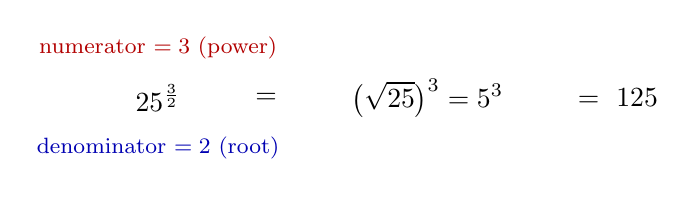
\begin{tikzpicture}[node distance=5mm and 7mm]
\node (e) {$\displaystyle 25^{\frac{3}{2}}$};
\node (eq) [right=of e] {$=$};
\node (mid) [right=of eq] {$\displaystyle \big(\sqrt{25}\big)^{3}=5^{3}$};
\node (res) [right=of mid] {$\displaystyle =\ 125$};
\node[red!70!black,font=\footnotesize,above=2pt of e] {numerator $=3$ (power)};
\node[blue!70!black,font=\footnotesize,below=2pt of e] {denominator $=2$ (root)};
\end{tikzpicture}
}
\end{center}
\small Fractional index: the \emph{denominator} gives the root, the \emph{numerator} gives the power.\normalsize

\medskip\hrule

\section*{Laws of Indices 18\quad\small\texttt{(a4-018)}}
\addcontentsline{toc}{section}{Laws of Indices 18 (a4-018)}
\textit{Difficulty: Foundation \quad\textbar\quad Marks: 2}

\question{Evaluate: \( 32^{\frac{2}{5}} \)}

\textbf{Worked solution.}

\textit{Step 1: Split the fractional exponent: fifth root first, then square.}
\[\begin{gathered}
32^{\frac{2}{5}} = \left(32^{\frac{1}{5}}\right)^2
\end{gathered}\]
The denominator 5 means take the fifth root; the numerator 2 means square.

\textit{Step 2: Evaluate the fifth root of 32.}
\[\begin{gathered}
32^{\frac{1}{5}} = 2
\end{gathered}\]
\( 2^5 = 32 \).

\textit{Step 3: Square the result.}
\[\begin{gathered}
2^2 = 4
\end{gathered}\]
\( 2 \times 2 = 4 \).

\begin{answerbox}
\textbf{Final answer:}\quad \(\displaystyle 4\)
\end{answerbox}
\textbf{Diagram.}

\begin{center}
\resizebox{\ifdim\width>\linewidth \linewidth\else \width\fi}{!}{%
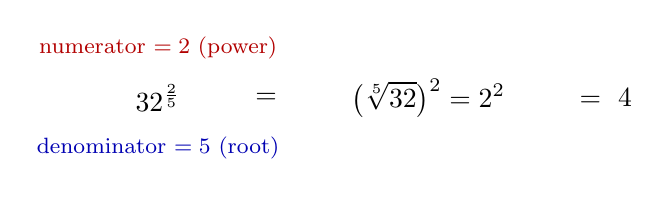
\begin{tikzpicture}[node distance=5mm and 7mm]
\node (e) {$\displaystyle 32^{\frac{2}{5}}$};
\node (eq) [right=of e] {$=$};
\node (mid) [right=of eq] {$\displaystyle \big(\sqrt[5]{32}\big)^{2}=2^{2}$};
\node (res) [right=of mid] {$\displaystyle =\ 4$};
\node[red!70!black,font=\footnotesize,above=2pt of e] {numerator $=2$ (power)};
\node[blue!70!black,font=\footnotesize,below=2pt of e] {denominator $=5$ (root)};
\end{tikzpicture}
}
\end{center}
\small Fractional index: the \emph{denominator} gives the root, the \emph{numerator} gives the power.\normalsize

\medskip\hrule

\section*{Laws of Indices 19\quad\small\texttt{(a4-019)}}
\addcontentsline{toc}{section}{Laws of Indices 19 (a4-019)}
\textit{Difficulty: Foundation \quad\textbar\quad Marks: 2}

\question{Evaluate: \( 4^{-\frac{1}{2}} \)}

\textbf{Worked solution.}

\textit{Step 1: Deal with the negative exponent by taking the reciprocal.}
\[\begin{gathered}
4^{-\frac{1}{2}} = \frac{1}{4^{\frac{1}{2}}}
\end{gathered}\]
A negative exponent means "one over": \( a^{-n} = \frac{1}{a^n} \).

\textit{Step 2: Evaluate the square root of 4.}
\[\begin{gathered}
4^{\frac{1}{2}} = 2
\end{gathered}\]
\( \sqrt{4} = 2 \).

\textit{Step 3: Write the final answer.}
\[\begin{gathered}
\frac{1}{2}
\end{gathered}\]
Substituting back gives \( \frac{1}{2} \).

\begin{answerbox}
\textbf{Final answer:}\quad \(\displaystyle \frac{1}{2}\)
\end{answerbox}
\textbf{Diagram.}

\begin{center}
\resizebox{\ifdim\width>\linewidth \linewidth\else \width\fi}{!}{%
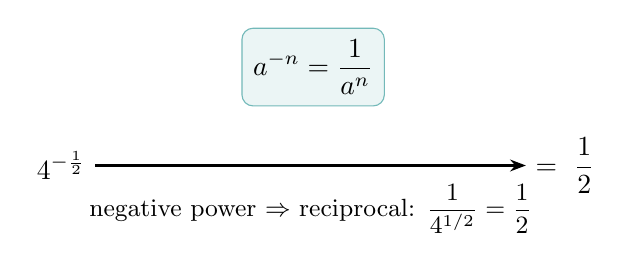
\begin{tikzpicture}[>={Stealth[length=2mm]}]
\node[draw=teal!55,rounded corners,fill=teal!8,inner sep=4pt] (rule) at (3.2,1.25) {$\displaystyle a^{-n}=\dfrac{1}{a^{n}}$};
\node (L) at (0,0) {$\displaystyle 4^{-\frac{1}{2}}$};
\node (R) at (6.4,0) {$\displaystyle =\ \dfrac{1}{2}$};
\draw[->,thick] (L) -- (R) node[midway,below=3pt,font=\small,align=center]{negative power $\Rightarrow$ reciprocal: $\dfrac{1}{4^{1/2}}=\dfrac{1}{2}$};
\end{tikzpicture}
}
\end{center}
\small Index-law card: the boxed general rule (teal) is applied to the expression.\normalsize

\medskip\hrule

\section*{Laws of Indices 20\quad\small\texttt{(a4-020)}}
\addcontentsline{toc}{section}{Laws of Indices 20 (a4-020)}
\textit{Difficulty: Foundation \quad\textbar\quad Marks: 3}

\question{Evaluate: \( 27^{-\frac{2}{3}} \)}

\textbf{Worked solution.}

\textit{Step 1: Deal with the negative sign by taking the reciprocal.}
\[\begin{gathered}
27^{-\frac{2}{3}} = \frac{1}{27^{\frac{2}{3}}}
\end{gathered}\]
Flip the base to make the exponent positive.

\textit{Step 2: Split the fractional exponent: cube root first, then square.}
\[\begin{gathered}
27^{\frac{2}{3}} = \left(27^{\frac{1}{3}}\right)^2 = 3^2 = 9
\end{gathered}\]
The cube root of 27 is 3, then \( 3^2 = 9 \).

\textit{Step 3: Write the final answer.}
\[\begin{gathered}
\frac{1}{9}
\end{gathered}\]
So \( 27^{-\frac{2}{3}} = \frac{1}{9} \).

\begin{answerbox}
\textbf{Final answer:}\quad \(\displaystyle \frac{1}{9}\)
\end{answerbox}
\textbf{Diagram.}

\begin{center}
\resizebox{\ifdim\width>\linewidth \linewidth\else \width\fi}{!}{%
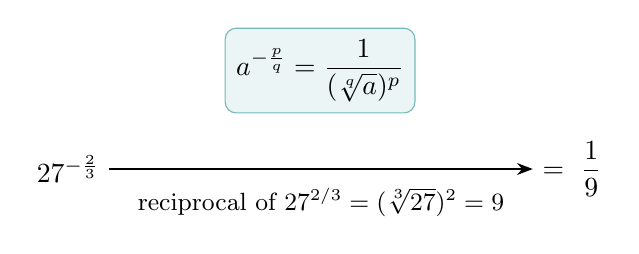
\begin{tikzpicture}[>={Stealth[length=2mm]}]
\node[draw=teal!55,rounded corners,fill=teal!8,inner sep=4pt] (rule) at (3.2,1.25) {$\displaystyle a^{-\frac{p}{q}}=\dfrac{1}{(\sqrt[q]{a})^{p}}$};
\node (L) at (0,0) {$\displaystyle 27^{-\frac{2}{3}}$};
\node (R) at (6.4,0) {$\displaystyle =\ \dfrac{1}{9}$};
\draw[->,thick] (L) -- (R) node[midway,below=3pt,font=\small,align=center]{reciprocal of $27^{2/3}=(\sqrt[3]{27})^{2}=9$};
\end{tikzpicture}
}
\end{center}
\small Index-law card: the boxed general rule (teal) is applied to the expression.\normalsize

\medskip\hrule

\section*{Laws of Indices 21\quad\small\texttt{(a4-021)}}
\addcontentsline{toc}{section}{Laws of Indices 21 (a4-021)}
\textit{Difficulty: Foundation \quad\textbar\quad Marks: 1}

\question{Express \( \frac{1}{m} \) as a power of \( m \).}

\textbf{Worked solution.}

\textit{"One over" a base is the same as that base raised to a negative power.}
\[\begin{gathered}
\frac{1}{m} = m^{-1}
\end{gathered}\]
By definition, \( a^{-1} = \frac{1}{a} \).

\begin{answerbox}
\textbf{Final answer:}\quad \(\displaystyle m^{-1}\)
\end{answerbox}
\textbf{Diagram.}

\begin{center}
\resizebox{\ifdim\width>\linewidth \linewidth\else \width\fi}{!}{%
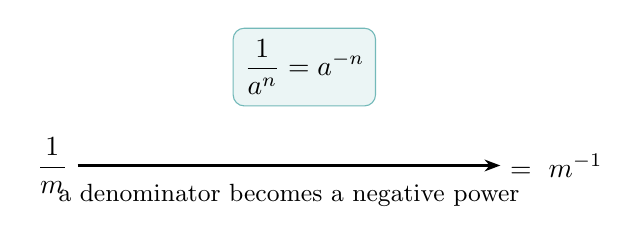
\begin{tikzpicture}[>={Stealth[length=2mm]}]
\node[draw=teal!55,rounded corners,fill=teal!8,inner sep=4pt] (rule) at (3.2,1.25) {$\displaystyle \dfrac{1}{a^{n}}=a^{-n}$};
\node (L) at (0,0) {$\displaystyle \dfrac{1}{m}$};
\node (R) at (6.4,0) {$\displaystyle =\ m^{-1}$};
\draw[->,thick] (L) -- (R) node[midway,below=3pt,font=\small,align=center]{a denominator becomes a negative power};
\end{tikzpicture}
}
\end{center}
\small Index-law card: the boxed general rule (teal) is applied to the expression.\normalsize

\medskip\hrule

\section*{Laws of Indices 22\quad\small\texttt{(a4-022)}}
\addcontentsline{toc}{section}{Laws of Indices 22 (a4-022)}
\textit{Difficulty: Foundation \quad\textbar\quad Marks: 1}

\question{Express \( \sqrt[3]{n} \) as a power of \( n \).}

\textbf{Worked solution.}

\textit{The cube root can be written as a fractional exponent.}
\[\begin{gathered}
\sqrt[3]{n} = n^{\frac{1}{3}}
\end{gathered}\]
The \( q \)th root of a number is the same as raising it to the power \( \frac{1}{q} \).

\begin{answerbox}
\textbf{Final answer:}\quad \(\displaystyle n^{\frac{1}{3}}\)
\end{answerbox}
\textbf{Diagram.}

\begin{center}
\resizebox{\ifdim\width>\linewidth \linewidth\else \width\fi}{!}{%
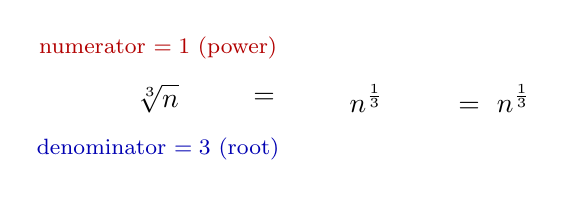
\begin{tikzpicture}[node distance=5mm and 7mm]
\node (e) {$\displaystyle \sqrt[3]{n}$};
\node (eq) [right=of e] {$=$};
\node (mid) [right=of eq] {$\displaystyle n^{\frac{1}{3}}$};
\node (res) [right=of mid] {$\displaystyle =\ n^{\frac{1}{3}}$};
\node[red!70!black,font=\footnotesize,above=2pt of e] {numerator $=1$ (power)};
\node[blue!70!black,font=\footnotesize,below=2pt of e] {denominator $=3$ (root)};
\end{tikzpicture}
}
\end{center}
\small Fractional index: the \emph{denominator} gives the root, the \emph{numerator} gives the power.\normalsize

\medskip\hrule

\section*{Laws of Indices 23\quad\small\texttt{(a4-023)}}
\addcontentsline{toc}{section}{Laws of Indices 23 (a4-023)}
\textit{Difficulty: Foundation \quad\textbar\quad Marks: 2}

\question{Express \( \frac{1}{\sqrt{t}} \) as a single power of \( t \).}

\textbf{Worked solution.}

\textit{Step 1: Rewrite the square root as a fractional exponent.}
\[\begin{gathered}
\frac{1}{\sqrt{t}} = \frac{1}{t^{\frac{1}{2}}}
\end{gathered}\]
\( \sqrt{t} = t^{\frac{1}{2}} \).

\textit{Step 2: Use the negative exponent rule to bring the base to the numerator.}
\[\begin{gathered}
t^{-\frac{1}{2}}
\end{gathered}\]
\( \frac{1}{a^n} = a^{-n} \).

\begin{answerbox}
\textbf{Final answer:}\quad \(\displaystyle t^{-\frac{1}{2}}\)
\end{answerbox}
\textbf{Diagram.}

\begin{center}
\resizebox{\ifdim\width>\linewidth \linewidth\else \width\fi}{!}{%
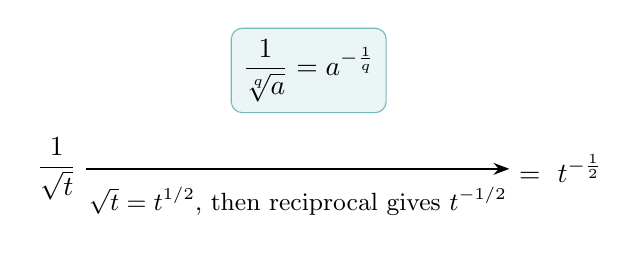
\begin{tikzpicture}[>={Stealth[length=2mm]}]
\node[draw=teal!55,rounded corners,fill=teal!8,inner sep=4pt] (rule) at (3.2,1.25) {$\displaystyle \dfrac{1}{\sqrt[q]{a}}=a^{-\frac{1}{q}}$};
\node (L) at (0,0) {$\displaystyle \dfrac{1}{\sqrt{t}}$};
\node (R) at (6.4,0) {$\displaystyle =\ t^{-\frac{1}{2}}$};
\draw[->,thick] (L) -- (R) node[midway,below=3pt,font=\small,align=center]{$\sqrt{t}=t^{1/2}$, then reciprocal gives $t^{-1/2}$};
\end{tikzpicture}
}
\end{center}
\small Index-law card: the boxed general rule (teal) is applied to the expression.\normalsize

\medskip\hrule

\section*{Laws of Indices 24\quad\small\texttt{(a4-024)}}
\addcontentsline{toc}{section}{Laws of Indices 24 (a4-024)}
\textit{Difficulty: Foundation \quad\textbar\quad Marks: 2}

\question{Express \( \left(\frac{1}{\sqrt[3]{x}}\right)^2 \) as a single power of \( x \).}

\textbf{Worked solution.}

\textit{Step 1: Rewrite the expression using index notation.}
\[\begin{gathered}
\left(\frac{1}{x^{\frac{1}{3}}}\right)^2 = \left(x^{-\frac{1}{3}}\right)^2
\end{gathered}\]
First convert the cube root, then move it to the numerator with a negative exponent.

\textit{Step 2: Apply the power-of-a-power law.}
\[\begin{gathered}
x^{-\frac{1}{3} \times 2} = x^{-\frac{2}{3}}
\end{gathered}\]
Multiply the exponents: \( -\frac{1}{3} \times 2 = -\frac{2}{3} \).

\begin{answerbox}
\textbf{Final answer:}\quad \(\displaystyle x^{-\frac{2}{3}}\)
\end{answerbox}
\textbf{Diagram.}

\begin{center}
\resizebox{\ifdim\width>\linewidth \linewidth\else \width\fi}{!}{%
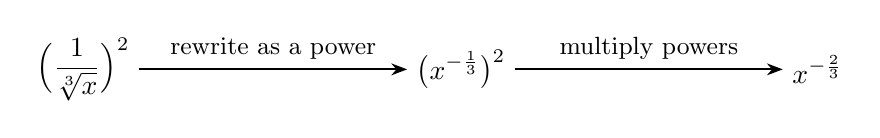
\begin{tikzpicture}[>={Stealth[length=2mm]},node distance=1.5cm and 3.4cm]
\node (s0) {$\displaystyle \Big(\dfrac{1}{\sqrt[3]{x}}\Big)^{2}$};
\node (s1) [right=of s0] {$\displaystyle \big(x^{-\frac{1}{3}}\big)^{2}$};
\node (s2) [right=of s1] {$\displaystyle x^{-\frac{2}{3}}$};
\draw[->,thick] (s0) -- (s1) node[midway,above,font=\small]{rewrite as a power};
\draw[->,thick] (s1) -- (s2) node[midway,above,font=\small]{multiply powers};
\end{tikzpicture}
}
\end{center}
\small Solution flow: each arrow applies one index law.\normalsize

\medskip\hrule

\section*{Laws of Indices 25\quad\small\texttt{(a4-025)}}
\addcontentsline{toc}{section}{Laws of Indices 25 (a4-025)}
\textit{Difficulty: Foundation \quad\textbar\quad Marks: 1}

\question{Simplify: \( (z^4)^{\frac{1}{2}} \)}

\textbf{Worked solution.}

\textit{Multiply the exponents using the power-of-a-power law.}
\[\begin{gathered}
z^{4 \times \frac{1}{2}} = z^{2}
\end{gathered}\]
\( 4 \times \frac{1}{2} = 2 \). Taking the square root of \( z^4 \) gives \( z^2 \).

\begin{answerbox}
\textbf{Final answer:}\quad \(\displaystyle z^{2}\)
\end{answerbox}
\textbf{Diagram.}

\begin{center}
\resizebox{\ifdim\width>\linewidth \linewidth\else \width\fi}{!}{%
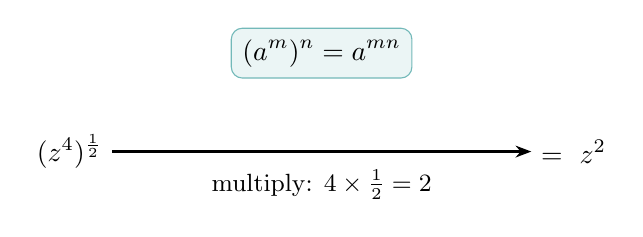
\begin{tikzpicture}[>={Stealth[length=2mm]}]
\node[draw=teal!55,rounded corners,fill=teal!8,inner sep=4pt] (rule) at (3.2,1.25) {$\displaystyle (a^{m})^{n}=a^{mn}$};
\node (L) at (0,0) {$\displaystyle (z^{4})^{\frac{1}{2}}$};
\node (R) at (6.4,0) {$\displaystyle =\ z^{2}$};
\draw[->,thick] (L) -- (R) node[midway,below=3pt,font=\small,align=center]{multiply: $4\times\tfrac12=2$};
\end{tikzpicture}
}
\end{center}
\small Index-law card: the boxed general rule (teal) is applied to the expression.\normalsize

\medskip\hrule

\section*{Laws of Indices 26\quad\small\texttt{(a4-026)}}
\addcontentsline{toc}{section}{Laws of Indices 26 (a4-026)}
\textit{Difficulty: Foundation \quad\textbar\quad Marks: 2}

\question{Simplify: \( (8^4)^{-\frac{1}{2}} \)}

\textbf{Worked solution.}

\textit{Step 1: Multiply the exponents.}
\[\begin{gathered}
8^{4 \times (-\frac{1}{2})} = 8^{-2}
\end{gathered}\]
\( 4 \times (-\frac{1}{2}) = -2 \).

\textit{Step 2: Deal with the negative exponent.}
\[\begin{gathered}
8^{-2} = \frac{1}{8^2} = \frac{1}{64}
\end{gathered}\]
\( 8^2 = 64 \), so the answer is \( \frac{1}{64} \).

\begin{answerbox}
\textbf{Final answer:}\quad \(\displaystyle \frac{1}{64}\)
\end{answerbox}
\textbf{Diagram.}

\begin{center}
\resizebox{\ifdim\width>\linewidth \linewidth\else \width\fi}{!}{%
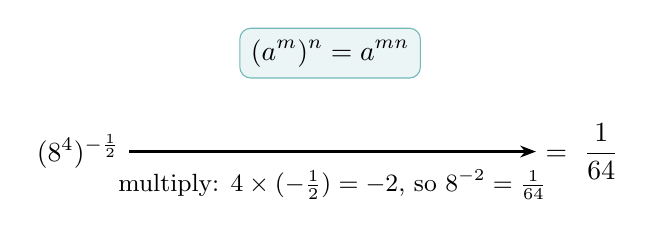
\begin{tikzpicture}[>={Stealth[length=2mm]}]
\node[draw=teal!55,rounded corners,fill=teal!8,inner sep=4pt] (rule) at (3.2,1.25) {$\displaystyle (a^{m})^{n}=a^{mn}$};
\node (L) at (0,0) {$\displaystyle (8^{4})^{-\frac{1}{2}}$};
\node (R) at (6.4,0) {$\displaystyle =\ \dfrac{1}{64}$};
\draw[->,thick] (L) -- (R) node[midway,below=3pt,font=\small,align=center]{multiply: $4\times(-\tfrac12)=-2$, so $8^{-2}=\tfrac{1}{64}$};
\end{tikzpicture}
}
\end{center}
\small Index-law card: the boxed general rule (teal) is applied to the expression.\normalsize

\medskip\hrule

\section*{Laws of Indices 27\quad\small\texttt{(a4-027)}}
\addcontentsline{toc}{section}{Laws of Indices 27 (a4-027)}
\textit{Difficulty: Foundation \quad\textbar\quad Marks: 2}

\question{Evaluate: \( \frac{2^3 \times 2}{2^5} \)}

\textbf{Worked solution.}

\textit{Step 1: Simplify the numerator using the multiplication law.}
\[\begin{gathered}
\frac{2^{3+1}}{2^5} = \frac{2^4}{2^5}
\end{gathered}\]
Remember \( 2 = 2^1 \), so \( 2^3 \times 2^1 = 2^4 \).

\textit{Step 2: Apply the division law.}
\[\begin{gathered}
2^{4-5} = 2^{-1}
\end{gathered}\]
Subtract the exponents.

\textit{Step 3: Evaluate.}
\[\begin{gathered}
2^{-1} = \frac{1}{2}
\end{gathered}\]
A power of \( -1 \) means the reciprocal.

\begin{answerbox}
\textbf{Final answer:}\quad \(\displaystyle \frac{1}{2}\)
\end{answerbox}
\textbf{Diagram.}

\begin{center}
\resizebox{\ifdim\width>\linewidth \linewidth\else \width\fi}{!}{%
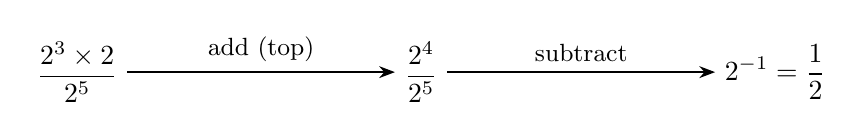
\begin{tikzpicture}[>={Stealth[length=2mm]},node distance=1.5cm and 3.4cm]
\node (s0) {$\displaystyle \dfrac{2^{3}\times 2}{2^{5}}$};
\node (s1) [right=of s0] {$\displaystyle \dfrac{2^{4}}{2^{5}}$};
\node (s2) [right=of s1] {$\displaystyle 2^{-1}=\dfrac{1}{2}$};
\draw[->,thick] (s0) -- (s1) node[midway,above,font=\small]{add (top)};
\draw[->,thick] (s1) -- (s2) node[midway,above,font=\small]{subtract};
\end{tikzpicture}
}
\end{center}
\small Solution flow: each arrow applies one index law.\normalsize

\medskip\hrule

\section*{Laws of Indices 28\quad\small\texttt{(a4-028)}}
\addcontentsline{toc}{section}{Laws of Indices 28 (a4-028)}
\textit{Difficulty: Foundation \quad\textbar\quad Marks: 2}

\question{Evaluate: \( \frac{7^3 \times 7^4}{7^6} \)}

\textbf{Worked solution.}

\textit{Step 1: Simplify the numerator by adding the exponents.}
\[\begin{gathered}
\frac{7^{3+4}}{7^6} = \frac{7^7}{7^6}
\end{gathered}\]
Both terms on top have the same base, so add the powers.

\textit{Step 2: Divide by subtracting exponents.}
\[\begin{gathered}
7^{7-6} = 7^1 = 7
\end{gathered}\]
\( 7 - 6 = 1 \), and \( 7^1 = 7 \).

\begin{answerbox}
\textbf{Final answer:}\quad \(\displaystyle 7\)
\end{answerbox}
\textbf{Diagram.}

\begin{center}
\resizebox{\ifdim\width>\linewidth \linewidth\else \width\fi}{!}{%
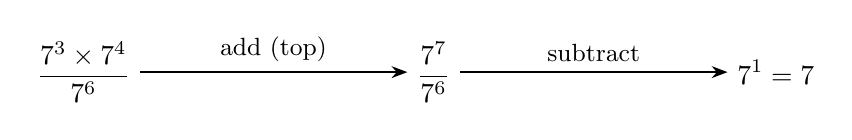
\begin{tikzpicture}[>={Stealth[length=2mm]},node distance=1.5cm and 3.4cm]
\node (s0) {$\displaystyle \dfrac{7^{3}\times 7^{4}}{7^{6}}$};
\node (s1) [right=of s0] {$\displaystyle \dfrac{7^{7}}{7^{6}}$};
\node (s2) [right=of s1] {$\displaystyle 7^{1}=7$};
\draw[->,thick] (s0) -- (s1) node[midway,above,font=\small]{add (top)};
\draw[->,thick] (s1) -- (s2) node[midway,above,font=\small]{subtract};
\end{tikzpicture}
}
\end{center}
\small Solution flow: each arrow applies one index law.\normalsize

\medskip\hrule

\section*{Laws of Indices 29\quad\small\texttt{(a4-029)}}
\addcontentsline{toc}{section}{Laws of Indices 29 (a4-029)}
\textit{Difficulty: Foundation \quad\textbar\quad Marks: 2}

\question{Evaluate: \( (3^2)^3 \div (3^1)^4 \)}

\textbf{Worked solution.}

\textit{Step 1: Apply the power-of-a-power law to both parts.}
\[\begin{gathered}
3^{2 \times 3} \div 3^{1 \times 4} = 3^6 \div 3^4
\end{gathered}\]
Multiply the exponents within each bracket.

\textit{Step 2: Subtract the exponents.}
\[\begin{gathered}
3^{6-4} = 3^2
\end{gathered}\]
\( 6 - 4 = 2 \).

\textit{Step 3: Evaluate.}
\[\begin{gathered}
3^2 = 9
\end{gathered}\]
\( 3 \times 3 = 9 \).

\begin{answerbox}
\textbf{Final answer:}\quad \(\displaystyle 9\)
\end{answerbox}
\textbf{Diagram.}

\begin{center}
\resizebox{\ifdim\width>\linewidth \linewidth\else \width\fi}{!}{%
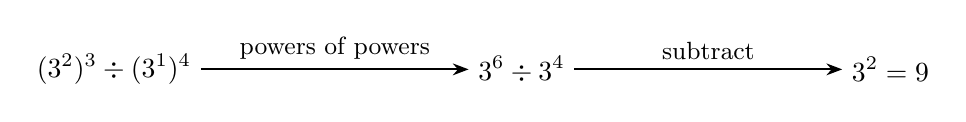
\begin{tikzpicture}[>={Stealth[length=2mm]},node distance=1.5cm and 3.4cm]
\node (s0) {$\displaystyle (3^{2})^{3}\div(3^{1})^{4}$};
\node (s1) [right=of s0] {$\displaystyle 3^{6}\div 3^{4}$};
\node (s2) [right=of s1] {$\displaystyle 3^{2}=9$};
\draw[->,thick] (s0) -- (s1) node[midway,above,font=\small]{powers of powers};
\draw[->,thick] (s1) -- (s2) node[midway,above,font=\small]{subtract};
\end{tikzpicture}
}
\end{center}
\small Solution flow: each arrow applies one index law.\normalsize

\medskip\hrule

\section*{Laws of Indices 30\quad\small\texttt{(a4-030)}}
\addcontentsline{toc}{section}{Laws of Indices 30 (a4-030)}
\textit{Difficulty: Foundation \quad\textbar\quad Marks: 3}

\question{Evaluate: \( \frac{(2^{\frac{1}{2}})^6 \times (2^{-1})^4}{(2^{-4})^{-2}} \)}

\textbf{Worked solution.}

\textit{Step 1: Apply the power-of-a-power law to each bracket.}
\[\begin{gathered}
\frac{2^{\frac{1}{2} \times 6} \times 2^{-1 \times 4}}{2^{-4 \times (-2)}} = \frac{2^3 \times 2^{-4}}{2^8}
\end{gathered}\]
Multiply each pair of exponents: \( \frac{1}{2} \times 6 = 3 \), \( -1 \times 4 = -4 \), \( -4 \times -2 = 8 \).

\textit{Step 2: Simplify the numerator by adding exponents.}
\[\begin{gathered}
\frac{2^{3+(-4)}}{2^8} = \frac{2^{-1}}{2^8}
\end{gathered}\]
\( 3 + (-4) = -1 \).

\textit{Step 3: Divide by subtracting the exponents.}
\[\begin{gathered}
2^{-1-8} = 2^{-9}
\end{gathered}\]
\( -1 - 8 = -9 \).

\textit{Step 4: Express as a fraction.}
\[\begin{gathered}
2^{-9} = \frac{1}{2^9} = \frac{1}{512}
\end{gathered}\]
\( 2^9 = 512 \).

\begin{answerbox}
\textbf{Final answer:}\quad \(\displaystyle \frac{1}{512}\)
\end{answerbox}
\textbf{Diagram.}

\begin{center}
\resizebox{\ifdim\width>\linewidth \linewidth\else \width\fi}{!}{%
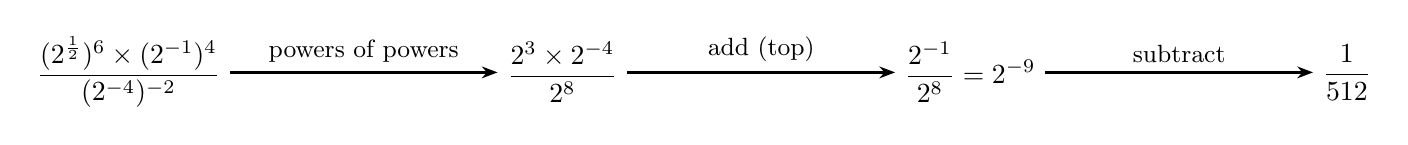
\begin{tikzpicture}[>={Stealth[length=2mm]},node distance=1.5cm and 3.4cm]
\node (s0) {$\displaystyle \dfrac{(2^{\frac12})^{6}\times(2^{-1})^{4}}{(2^{-4})^{-2}}$};
\node (s1) [right=of s0] {$\displaystyle \dfrac{2^{3}\times 2^{-4}}{2^{8}}$};
\node (s2) [right=of s1] {$\displaystyle \dfrac{2^{-1}}{2^{8}}=2^{-9}$};
\node (s3) [right=of s2] {$\displaystyle \dfrac{1}{512}$};
\draw[->,thick] (s0) -- (s1) node[midway,above,font=\small]{powers of powers};
\draw[->,thick] (s1) -- (s2) node[midway,above,font=\small]{add (top)};
\draw[->,thick] (s2) -- (s3) node[midway,above,font=\small]{subtract};
\end{tikzpicture}
}
\end{center}
\small Solution flow: each arrow applies one index law.\normalsize

\medskip\hrule

\section*{Laws of Indices 31\quad\small\texttt{(a4-031)}}
\addcontentsline{toc}{section}{Laws of Indices 31 (a4-031)}
\textit{Difficulty: Foundation \quad\textbar\quad Marks: 2}

\question{Simplify, leaving your answer as a single power of \( a \): \( \frac{a^5 \times a^3}{a^2} \)}

\textbf{Worked solution.}

\textit{Step 1: Simplify the numerator by adding the exponents.}
\[\begin{gathered}
\frac{a^{5+3}}{a^2} = \frac{a^8}{a^2}
\end{gathered}\]
Add the exponents on top: \( 5 + 3 = 8 \).

\textit{Step 2: Divide by subtracting the exponents.}
\[\begin{gathered}
a^{8-2} = a^6
\end{gathered}\]
\( 8 - 2 = 6 \).

\begin{answerbox}
\textbf{Final answer:}\quad \(\displaystyle a^6\)
\end{answerbox}
\textbf{Diagram.}

\begin{center}
\resizebox{\ifdim\width>\linewidth \linewidth\else \width\fi}{!}{%
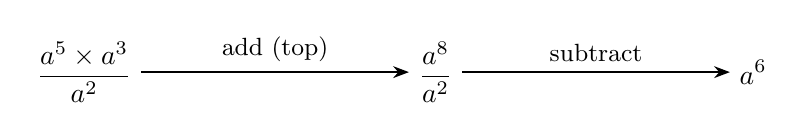
\begin{tikzpicture}[>={Stealth[length=2mm]},node distance=1.5cm and 3.4cm]
\node (s0) {$\displaystyle \dfrac{a^{5}\times a^{3}}{a^{2}}$};
\node (s1) [right=of s0] {$\displaystyle \dfrac{a^{8}}{a^{2}}$};
\node (s2) [right=of s1] {$\displaystyle a^{6}$};
\draw[->,thick] (s0) -- (s1) node[midway,above,font=\small]{add (top)};
\draw[->,thick] (s1) -- (s2) node[midway,above,font=\small]{subtract};
\end{tikzpicture}
}
\end{center}
\small Solution flow: each arrow applies one index law.\normalsize

\medskip\hrule

\section*{Laws of Indices 32\quad\small\texttt{(a4-032)}}
\addcontentsline{toc}{section}{Laws of Indices 32 (a4-032)}
\textit{Difficulty: Foundation \quad\textbar\quad Marks: 2}

\question{Simplify: \( \frac{c^4 d^{\frac{1}{2}}}{c^{-1} d^3} \)}

\textbf{Worked solution.}

\textit{Step 1: Apply the division law to each variable separately.}
\[\begin{gathered}
c^{4-(-1)} \times d^{\frac{1}{2}-3}
\end{gathered}\]
Subtract the exponent on the bottom from the exponent on the top for each base.

\textit{Step 2: Simplify each exponent.}
\[\begin{gathered}
c^{5} d^{-\frac{5}{2}}
\end{gathered}\]
\( 4 - (-1) = 5 \) and \( \frac{1}{2} - 3 = -\frac{5}{2} \).

\begin{answerbox}
\textbf{Final answer:}\quad \(\displaystyle c^{5} d^{-\frac{5}{2}}\)
\end{answerbox}
\textbf{Diagram.}

\begin{center}
\resizebox{\ifdim\width>\linewidth \linewidth\else \width\fi}{!}{%
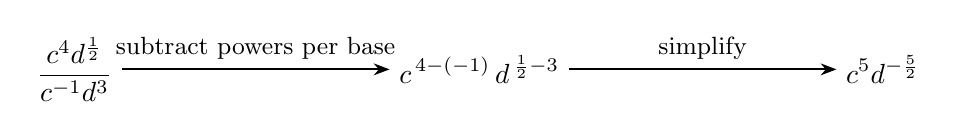
\begin{tikzpicture}[>={Stealth[length=2mm]},node distance=1.5cm and 3.4cm]
\node (s0) {$\displaystyle \dfrac{c^{4}d^{\frac12}}{c^{-1}d^{3}}$};
\node (s1) [right=of s0] {$\displaystyle c^{\,4-(-1)}\,d^{\,\frac12-3}$};
\node (s2) [right=of s1] {$\displaystyle c^{5}d^{-\frac{5}{2}}$};
\draw[->,thick] (s0) -- (s1) node[midway,above,font=\small]{subtract powers per base};
\draw[->,thick] (s1) -- (s2) node[midway,above,font=\small]{simplify};
\end{tikzpicture}
}
\end{center}
\small Solution flow: each arrow applies one index law.\normalsize

\medskip\hrule

\section*{Laws of Indices 33\quad\small\texttt{(a4-033)}}
\addcontentsline{toc}{section}{Laws of Indices 33 (a4-033)}
\textit{Difficulty: Foundation \quad\textbar\quad Marks: 2}

\question{Simplify: \( \frac{12y z^{\frac{1}{3}}}{4y z^{\frac{1}{2}}} \)}

\textbf{Worked solution.}

\textit{Step 1: Divide the numerical coefficients and apply the division law to each variable.}
\[\begin{gathered}
\frac{12}{4} \times y^{1-1} \times z^{\frac{1}{3}-\frac{1}{2}}
\end{gathered}\]
Deal with the numbers, the \( y \) terms, and the \( z \) terms separately.

\textit{Step 2: Simplify each part.}
\[\begin{gathered}
3 \times y^0 \times z^{-\frac{1}{6}} = 3z^{-\frac{1}{6}}
\end{gathered}\]
\( \frac{12}{4} = 3 \), \( y^0 = 1 \), and \( \frac{1}{3} - \frac{1}{2} = \frac{2-3}{6} = -\frac{1}{6} \).

\begin{answerbox}
\textbf{Final answer:}\quad \(\displaystyle 3z^{-\frac{1}{6}}\)
\end{answerbox}
\textbf{Diagram.}

\begin{center}
\resizebox{\ifdim\width>\linewidth \linewidth\else \width\fi}{!}{%
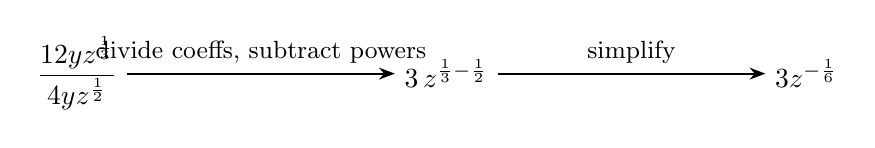
\begin{tikzpicture}[>={Stealth[length=2mm]},node distance=1.5cm and 3.4cm]
\node (s0) {$\displaystyle \dfrac{12yz^{\frac13}}{4yz^{\frac12}}$};
\node (s1) [right=of s0] {$\displaystyle 3\,z^{\frac13-\frac12}$};
\node (s2) [right=of s1] {$\displaystyle 3z^{-\frac{1}{6}}$};
\draw[->,thick] (s0) -- (s1) node[midway,above,font=\small]{divide coeffs, subtract powers};
\draw[->,thick] (s1) -- (s2) node[midway,above,font=\small]{simplify};
\end{tikzpicture}
}
\end{center}
\small Solution flow: each arrow applies one index law.\normalsize

\medskip\hrule

\section*{Laws of Indices 34\quad\small\texttt{(a4-034)}}
\addcontentsline{toc}{section}{Laws of Indices 34 (a4-034)}
\textit{Difficulty: Foundation \quad\textbar\quad Marks: 2}

\question{Simplify: \( (ab^2)^3 \)}

\textbf{Worked solution.}

\textit{Step 1: Raise each factor inside the bracket to the power 3.}
\[\begin{gathered}
a^3 \times (b^2)^3
\end{gathered}\]
When a product is raised to a power, each factor is raised to that power: \( (ab)^n = a^n b^n \).

\textit{Step 2: Apply the power-of-a-power law to \( (b^2)^3 \).}
\[\begin{gathered}
a^3 b^{6}
\end{gathered}\]
\( 2 \times 3 = 6 \).

\begin{answerbox}
\textbf{Final answer:}\quad \(\displaystyle a^3 b^{6}\)
\end{answerbox}
\textbf{Diagram.}

\begin{center}
\resizebox{\ifdim\width>\linewidth \linewidth\else \width\fi}{!}{%
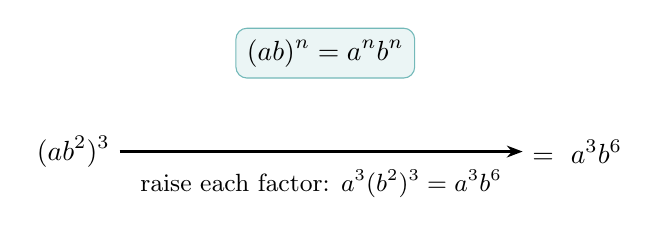
\begin{tikzpicture}[>={Stealth[length=2mm]}]
\node[draw=teal!55,rounded corners,fill=teal!8,inner sep=4pt] (rule) at (3.2,1.25) {$\displaystyle (ab)^{n}=a^{n}b^{n}$};
\node (L) at (0,0) {$\displaystyle (ab^{2})^{3}$};
\node (R) at (6.4,0) {$\displaystyle =\ a^{3}b^{6}$};
\draw[->,thick] (L) -- (R) node[midway,below=3pt,font=\small,align=center]{raise each factor: $a^{3}(b^{2})^{3}=a^{3}b^{6}$};
\end{tikzpicture}
}
\end{center}
\small Index-law card: the boxed general rule (teal) is applied to the expression.\normalsize

\medskip\hrule

\section*{Laws of Indices 35\quad\small\texttt{(a4-035)}}
\addcontentsline{toc}{section}{Laws of Indices 35 (a4-035)}
\textit{Difficulty: Foundation \quad\textbar\quad Marks: 2}

\question{Simplify: \( (mn^{\frac{1}{2}})^4 \)}

\textbf{Worked solution.}

\textit{Step 1: Raise each factor inside the bracket to the power 4.}
\[\begin{gathered}
m^4 \times (n^{\frac{1}{2}})^4
\end{gathered}\]
Distribute the exponent across the product.

\textit{Step 2: Apply the power-of-a-power law.}
\[\begin{gathered}
m^4 n^{\frac{1}{2} \times 4} = m^4 n^{2}
\end{gathered}\]
\( \frac{1}{2} \times 4 = 2 \).

\begin{answerbox}
\textbf{Final answer:}\quad \(\displaystyle m^4 n^{2}\)
\end{answerbox}
\textbf{Diagram.}

\begin{center}
\resizebox{\ifdim\width>\linewidth \linewidth\else \width\fi}{!}{%
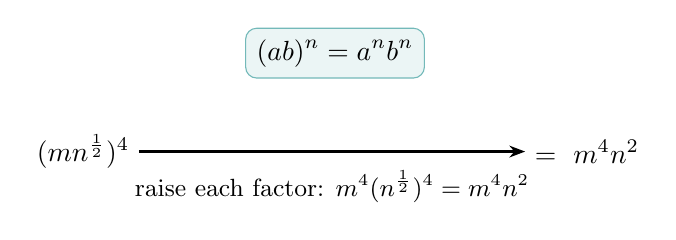
\begin{tikzpicture}[>={Stealth[length=2mm]}]
\node[draw=teal!55,rounded corners,fill=teal!8,inner sep=4pt] (rule) at (3.2,1.25) {$\displaystyle (ab)^{n}=a^{n}b^{n}$};
\node (L) at (0,0) {$\displaystyle (mn^{\frac{1}{2}})^{4}$};
\node (R) at (6.4,0) {$\displaystyle =\ m^{4}n^{2}$};
\draw[->,thick] (L) -- (R) node[midway,below=3pt,font=\small,align=center]{raise each factor: $m^{4}(n^{\frac12})^{4}=m^{4}n^{2}$};
\end{tikzpicture}
}
\end{center}
\small Index-law card: the boxed general rule (teal) is applied to the expression.\normalsize

\medskip\hrule

\section*{Laws of Indices 36\quad\small\texttt{(a4-036)}}
\addcontentsline{toc}{section}{Laws of Indices 36 (a4-036)}
\textit{Difficulty: Foundation \quad\textbar\quad Marks: 2}

\question{Simplify: \( \frac{p^3 q^4}{p^5 q} \)}

\textbf{Worked solution.}

\textit{Step 1: Apply the division law to each variable separately.}
\[\begin{gathered}
p^{3-5} \times q^{4-1}
\end{gathered}\]
Subtract bottom exponent from top exponent for each base.

\textit{Step 2: Simplify.}
\[\begin{gathered}
p^{-2} q^{3}
\end{gathered}\]
\( 3 - 5 = -2 \) and \( 4 - 1 = 3 \).

\begin{answerbox}
\textbf{Final answer:}\quad \(\displaystyle p^{-2} q^{3}\)
\end{answerbox}
\textbf{Diagram.}

\begin{center}
\resizebox{\ifdim\width>\linewidth \linewidth\else \width\fi}{!}{%
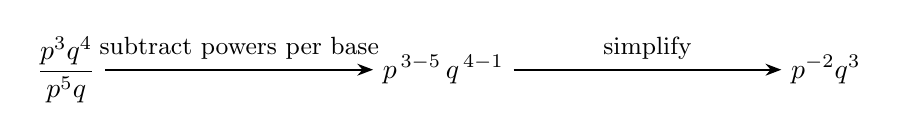
\begin{tikzpicture}[>={Stealth[length=2mm]},node distance=1.5cm and 3.4cm]
\node (s0) {$\displaystyle \dfrac{p^{3}q^{4}}{p^{5}q}$};
\node (s1) [right=of s0] {$\displaystyle p^{\,3-5}\,q^{\,4-1}$};
\node (s2) [right=of s1] {$\displaystyle p^{-2}q^{3}$};
\draw[->,thick] (s0) -- (s1) node[midway,above,font=\small]{subtract powers per base};
\draw[->,thick] (s1) -- (s2) node[midway,above,font=\small]{simplify};
\end{tikzpicture}
}
\end{center}
\small Solution flow: each arrow applies one index law.\normalsize

\medskip\hrule

\section*{Laws of Indices 37\quad\small\texttt{(a4-037)}}
\addcontentsline{toc}{section}{Laws of Indices 37 (a4-037)}
\textit{Difficulty: Foundation \quad\textbar\quad Marks: 3}

\question{Evaluate: \( (4^{-\frac{1}{2}})^2 \times (4^{-1})^{\frac{1}{2}} \)}

\textbf{Worked solution.}

\textit{Step 1: Apply the power-of-a-power law to each bracket.}
\[\begin{gathered}
4^{-\frac{1}{2} \times 2} \times 4^{-1 \times \frac{1}{2}} = 4^{-1} \times 4^{-\frac{1}{2}}
\end{gathered}\]
\( -\frac{1}{2} \times 2 = -1 \) and \( -1 \times \frac{1}{2} = -\frac{1}{2} \).

\textit{Step 2: Add the exponents since the bases are the same.}
\[\begin{gathered}
4^{-1 + (-\frac{1}{2})} = 4^{-\frac{3}{2}}
\end{gathered}\]
\( -1 - \frac{1}{2} = -\frac{3}{2} \).

\textit{Step 3: Evaluate \( 4^{-\frac{3}{2}} \).}
\[\begin{gathered}
\frac{1}{4^{\frac{3}{2}}} = \frac{1}{(\sqrt{4})^3} = \frac{1}{2^3} = \frac{1}{8}
\end{gathered}\]
Take the reciprocal, then root-before-power: \( \sqrt{4} = 2 \), then \( 2^3 = 8 \).

\begin{answerbox}
\textbf{Final answer:}\quad \(\displaystyle \frac{1}{8}\)
\end{answerbox}
\textbf{Diagram.}

\begin{center}
\resizebox{\ifdim\width>\linewidth \linewidth\else \width\fi}{!}{%
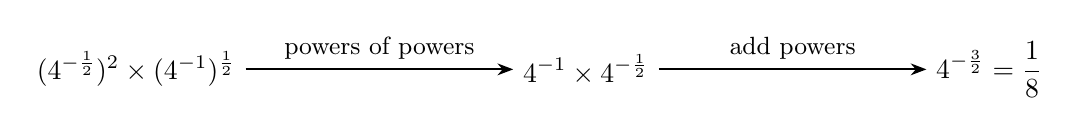
\begin{tikzpicture}[>={Stealth[length=2mm]},node distance=1.5cm and 3.4cm]
\node (s0) {$\displaystyle (4^{-\frac12})^{2}\times(4^{-1})^{\frac12}$};
\node (s1) [right=of s0] {$\displaystyle 4^{-1}\times 4^{-\frac12}$};
\node (s2) [right=of s1] {$\displaystyle 4^{-\frac{3}{2}}=\dfrac{1}{8}$};
\draw[->,thick] (s0) -- (s1) node[midway,above,font=\small]{powers of powers};
\draw[->,thick] (s1) -- (s2) node[midway,above,font=\small]{add powers};
\end{tikzpicture}
}
\end{center}
\small Solution flow: each arrow applies one index law.\normalsize

\medskip\hrule

\section*{Laws of Indices 38\quad\small\texttt{(a4-038)}}
\addcontentsline{toc}{section}{Laws of Indices 38 (a4-038)}
\textit{Difficulty: Foundation \quad\textbar\quad Marks: 2}

\question{Find the value of \( x \): \( 4^x = \sqrt{4} \)}

\textbf{Worked solution.}

\textit{Step 1: Rewrite the right-hand side using index notation.}
\[\begin{gathered}
\sqrt{4} = 4^{\frac{1}{2}}
\end{gathered}\]
A square root is a power of \( \frac{1}{2} \).

\textit{Step 2: Compare the exponents since the bases are equal.}
\[\begin{gathered}
4^x = 4^{\frac{1}{2}} \implies x = \frac{1}{2}
\end{gathered}\]
If \( a^x = a^y \) then \( x = y \).

\begin{answerbox}
\textbf{Final answer:}\quad \(\displaystyle x = \frac{1}{2}\)
\end{answerbox}
\textbf{Diagram.}

\begin{center}
\resizebox{\ifdim\width>\linewidth \linewidth\else \width\fi}{!}{%
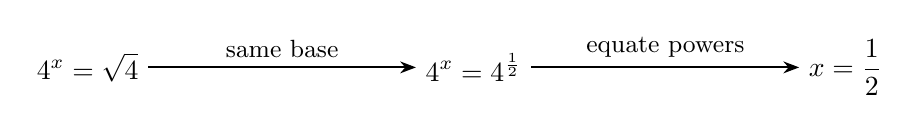
\begin{tikzpicture}[>={Stealth[length=2mm]},node distance=1.5cm and 3.4cm]
\node (s0) {$\displaystyle 4^{x}=\sqrt{4}$};
\node (s1) [right=of s0] {$\displaystyle 4^{x}=4^{\frac{1}{2}}$};
\node (s2) [right=of s1] {$\displaystyle x=\dfrac{1}{2}$};
\draw[->,thick] (s0) -- (s1) node[midway,above,font=\small]{same base};
\draw[->,thick] (s1) -- (s2) node[midway,above,font=\small]{equate powers};
\end{tikzpicture}
}
\end{center}
\small Solution flow: each arrow applies one index law.\normalsize

\medskip\hrule

\section*{Laws of Indices 39\quad\small\texttt{(a4-039)}}
\addcontentsline{toc}{section}{Laws of Indices 39 (a4-039)}
\textit{Difficulty: Foundation \quad\textbar\quad Marks: 3}

\question{Find the value of \( x \): \( 9^x = \frac{1}{3} \)}

\textbf{Worked solution.}

\textit{Step 1: Write both sides with the same base. Since \( 9 = 3^2 \), rewrite the left-hand side.}
\[\begin{gathered}
(3^2)^x = 3^{-1}
\end{gathered}\]
\( \frac{1}{3} = 3^{-1} \) and \( 9 = 3^2 \).

\textit{Step 2: Simplify the left-hand side using the power-of-a-power law.}
\[\begin{gathered}
3^{2x} = 3^{-1}
\end{gathered}\]
\( (3^2)^x = 3^{2x} \).

\textit{Step 3: Since the bases are equal, set the exponents equal and solve.}
\[\begin{gathered}
2x = -1 \implies x = -\frac{1}{2}
\end{gathered}\]
Divide both sides by 2.

\begin{answerbox}
\textbf{Final answer:}\quad \(\displaystyle x = -\frac{1}{2}\)
\end{answerbox}
\textbf{Diagram.}

\begin{center}
\resizebox{\ifdim\width>\linewidth \linewidth\else \width\fi}{!}{%
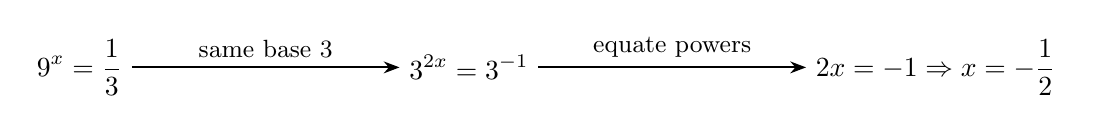
\begin{tikzpicture}[>={Stealth[length=2mm]},node distance=1.5cm and 3.4cm]
\node (s0) {$\displaystyle 9^{x}=\dfrac{1}{3}$};
\node (s1) [right=of s0] {$\displaystyle 3^{2x}=3^{-1}$};
\node (s2) [right=of s1] {$\displaystyle 2x=-1\Rightarrow x=-\dfrac{1}{2}$};
\draw[->,thick] (s0) -- (s1) node[midway,above,font=\small]{same base $3$};
\draw[->,thick] (s1) -- (s2) node[midway,above,font=\small]{equate powers};
\end{tikzpicture}
}
\end{center}
\small Solution flow: each arrow applies one index law.\normalsize

\medskip\hrule

\section*{Laws of Indices 40\quad\small\texttt{(a4-040)}}
\addcontentsline{toc}{section}{Laws of Indices 40 (a4-040)}
\textit{Difficulty: Foundation \quad\textbar\quad Marks: 2}

\question{Find the value of \( x \): \( \sqrt{5} \times 5^3 = 5^x \)}

\textbf{Worked solution.}

\textit{Step 1: Rewrite \( \sqrt{5} \) as a power of 5.}
\[\begin{gathered}
5^{\frac{1}{2}} \times 5^3 = 5^x
\end{gathered}\]
\( \sqrt{5} = 5^{\frac{1}{2}} \).

\textit{Step 2: Add the exponents on the left-hand side.}
\[\begin{gathered}
5^{\frac{1}{2}+3} = 5^{\frac{7}{2}} = 5^x
\end{gathered}\]
\( \frac{1}{2} + 3 = \frac{1}{2} + \frac{6}{2} = \frac{7}{2} \).

\textit{Step 3: Compare exponents.}
\[\begin{gathered}
x = \frac{7}{2}
\end{gathered}\]
Both sides have base 5, so the exponents must be equal.

\begin{answerbox}
\textbf{Final answer:}\quad \(\displaystyle x = \frac{7}{2}\)
\end{answerbox}
\textbf{Diagram.}

\begin{center}
\resizebox{\ifdim\width>\linewidth \linewidth\else \width\fi}{!}{%
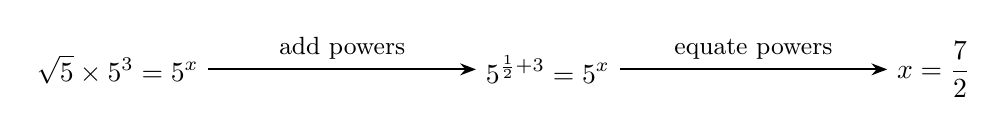
\begin{tikzpicture}[>={Stealth[length=2mm]},node distance=1.5cm and 3.4cm]
\node (s0) {$\displaystyle \sqrt{5}\times 5^{3}=5^{x}$};
\node (s1) [right=of s0] {$\displaystyle 5^{\frac{1}{2}+3}=5^{x}$};
\node (s2) [right=of s1] {$\displaystyle x=\dfrac{7}{2}$};
\draw[->,thick] (s0) -- (s1) node[midway,above,font=\small]{add powers};
\draw[->,thick] (s1) -- (s2) node[midway,above,font=\small]{equate powers};
\end{tikzpicture}
}
\end{center}
\small Solution flow: each arrow applies one index law.\normalsize

\medskip\hrule

\section*{Laws of Indices 41\quad\small\texttt{(a4-041)}}
\addcontentsline{toc}{section}{Laws of Indices 41 (a4-041)}
\textit{Difficulty: Foundation \quad\textbar\quad Marks: 1}

\question{Simplify, leaving your answer as a power: \( 10^6 \times 10^{-2} \)}

\textbf{Worked solution.}

\textit{Step 1: Add the exponents since the bases are the same.}
\[\begin{gathered}
10^{6+(-2)} = 10^{6-2}
\end{gathered}\]
The multiplication law says \( a^m \times a^n = a^{m+n} \).

\textit{Step 2: Simplify the exponent.}
\[\begin{gathered}
10^{4}
\end{gathered}\]
\( 6 - 2 = 4 \).

\begin{answerbox}
\textbf{Final answer:}\quad \(\displaystyle 10^{4}\)
\end{answerbox}
\textbf{Diagram.}

\begin{center}
\resizebox{\ifdim\width>\linewidth \linewidth\else \width\fi}{!}{%
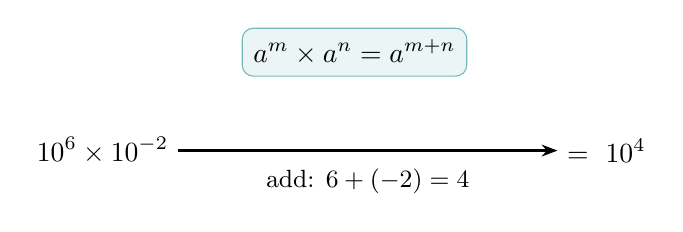
\begin{tikzpicture}[>={Stealth[length=2mm]}]
\node[draw=teal!55,rounded corners,fill=teal!8,inner sep=4pt] (rule) at (3.2,1.25) {$\displaystyle a^{m}\times a^{n}=a^{m+n}$};
\node (L) at (0,0) {$\displaystyle 10^{6}\times 10^{-2}$};
\node (R) at (6.4,0) {$\displaystyle =\ 10^{4}$};
\draw[->,thick] (L) -- (R) node[midway,below=3pt,font=\small,align=center]{add: $6+(-2)=4$};
\end{tikzpicture}
}
\end{center}
\small Index-law card: the boxed general rule (teal) is applied to the expression.\normalsize

\medskip\hrule

\section*{Laws of Indices 42\quad\small\texttt{(a4-042)}}
\addcontentsline{toc}{section}{Laws of Indices 42 (a4-042)}
\textit{Difficulty: Foundation \quad\textbar\quad Marks: 1}

\question{Evaluate: \( 64^{\frac{1}{3}} \)}

\textbf{Worked solution.}

\textit{Step 1: Recognise that a power of \( \frac{1}{3} \) means the cube root.}
\[\begin{gathered}
64^{\frac{1}{3}} = \sqrt[3]{64}
\end{gathered}\]
\( a^{\frac{1}{3}} = \sqrt[3]{a} \).

\textit{Step 2: Evaluate the cube root.}
\[\begin{gathered}
4
\end{gathered}\]
\( 4 \times 4 \times 4 = 64 \), so \( \sqrt[3]{64} = 4 \).

\begin{answerbox}
\textbf{Final answer:}\quad \(\displaystyle 4\)
\end{answerbox}
\textbf{Diagram.}

\begin{center}
\resizebox{\ifdim\width>\linewidth \linewidth\else \width\fi}{!}{%
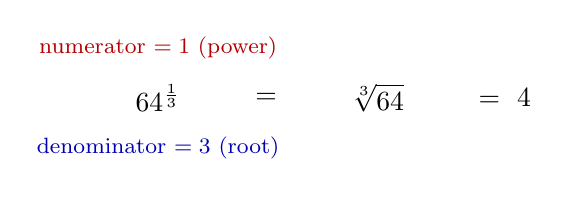
\begin{tikzpicture}[node distance=5mm and 7mm]
\node (e) {$\displaystyle 64^{\frac{1}{3}}$};
\node (eq) [right=of e] {$=$};
\node (mid) [right=of eq] {$\displaystyle \sqrt[3]{64}$};
\node (res) [right=of mid] {$\displaystyle =\ 4$};
\node[red!70!black,font=\footnotesize,above=2pt of e] {numerator $=1$ (power)};
\node[blue!70!black,font=\footnotesize,below=2pt of e] {denominator $=3$ (root)};
\end{tikzpicture}
}
\end{center}
\small Fractional index: the \emph{denominator} gives the root, the \emph{numerator} gives the power.\normalsize

\medskip\hrule

\section*{Laws of Indices 43\quad\small\texttt{(a4-043)}}
\addcontentsline{toc}{section}{Laws of Indices 43 (a4-043)}
\textit{Difficulty: Foundation \quad\textbar\quad Marks: 2}

\question{Simplify, leaving your answer as a single power of \( w \): \( w^7 \div w^{-3} \)}

\textbf{Worked solution.}

\textit{Step 1: Subtract the exponents using the division law.}
\[\begin{gathered}
w^{7-(-3)}
\end{gathered}\]
\( a^m \div a^n = a^{m-n} \). Be careful: subtracting a negative is the same as adding.

\textit{Step 2: Simplify the exponent.}
\[\begin{gathered}
w^{10}
\end{gathered}\]
\( 7 - (-3) = 7 + 3 = 10 \).

\begin{answerbox}
\textbf{Final answer:}\quad \(\displaystyle w^{10}\)
\end{answerbox}
\textbf{Diagram.}

\begin{center}
\resizebox{\ifdim\width>\linewidth \linewidth\else \width\fi}{!}{%
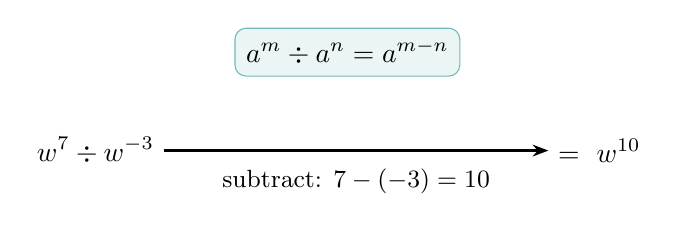
\begin{tikzpicture}[>={Stealth[length=2mm]}]
\node[draw=teal!55,rounded corners,fill=teal!8,inner sep=4pt] (rule) at (3.2,1.25) {$\displaystyle a^{m}\div a^{n}=a^{m-n}$};
\node (L) at (0,0) {$\displaystyle w^{7}\div w^{-3}$};
\node (R) at (6.4,0) {$\displaystyle =\ w^{10}$};
\draw[->,thick] (L) -- (R) node[midway,below=3pt,font=\small,align=center]{subtract: $7-(-3)=10$};
\end{tikzpicture}
}
\end{center}
\small Index-law card: the boxed general rule (teal) is applied to the expression.\normalsize

\medskip\hrule

\section*{Laws of Indices 44\quad\small\texttt{(a4-044)}}
\addcontentsline{toc}{section}{Laws of Indices 44 (a4-044)}
\textit{Difficulty: Foundation \quad\textbar\quad Marks: 2}

\question{Evaluate: \( 100^{\frac{3}{2}} \)}

\textbf{Worked solution.}

\textit{Step 1: Split the fractional exponent: square root first, then cube.}
\[\begin{gathered}
100^{\frac{3}{2}} = \left(100^{\frac{1}{2}}\right)^3
\end{gathered}\]
The denominator 2 means square root; the numerator 3 means cube.

\textit{Step 2: Take the square root of 100.}
\[\begin{gathered}
100^{\frac{1}{2}} = 10
\end{gathered}\]
\( 10 \times 10 = 100 \).

\textit{Step 3: Cube the result.}
\[\begin{gathered}
10^3 = 1000
\end{gathered}\]
\( 10 \times 10 \times 10 = 1000 \).

\begin{answerbox}
\textbf{Final answer:}\quad \(\displaystyle 1000\)
\end{answerbox}
\textbf{Diagram.}

\begin{center}
\resizebox{\ifdim\width>\linewidth \linewidth\else \width\fi}{!}{%
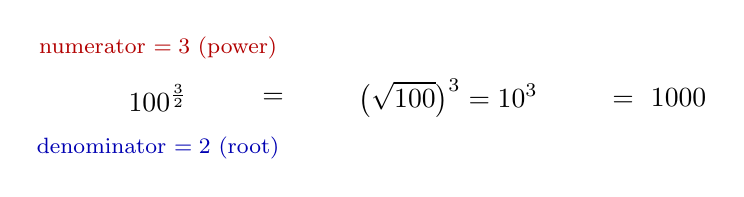
\begin{tikzpicture}[node distance=5mm and 7mm]
\node (e) {$\displaystyle 100^{\frac{3}{2}}$};
\node (eq) [right=of e] {$=$};
\node (mid) [right=of eq] {$\displaystyle \big(\sqrt{100}\big)^{3}=10^{3}$};
\node (res) [right=of mid] {$\displaystyle =\ 1000$};
\node[red!70!black,font=\footnotesize,above=2pt of e] {numerator $=3$ (power)};
\node[blue!70!black,font=\footnotesize,below=2pt of e] {denominator $=2$ (root)};
\end{tikzpicture}
}
\end{center}
\small Fractional index: the \emph{denominator} gives the root, the \emph{numerator} gives the power.\normalsize

\medskip\hrule

\section*{Laws of Indices 45\quad\small\texttt{(a4-045)}}
\addcontentsline{toc}{section}{Laws of Indices 45 (a4-045)}
\textit{Difficulty: Foundation \quad\textbar\quad Marks: 2}

\question{Simplify: \( \frac{(3^2)^4}{3^5} \)}

\textbf{Worked solution.}

\textit{Step 1: Apply the power-of-a-power law to the numerator.}
\[\begin{gathered}
\frac{3^{2 \times 4}}{3^5} = \frac{3^8}{3^5}
\end{gathered}\]
Multiply the exponents: \( 2 \times 4 = 8 \).

\textit{Step 2: Apply the division law.}
\[\begin{gathered}
3^{8-5} = 3^3
\end{gathered}\]
\( 8 - 5 = 3 \).

\textit{Step 3: Evaluate.}
\[\begin{gathered}
3^3 = 27
\end{gathered}\]
\( 3 \times 3 \times 3 = 27 \).

\begin{answerbox}
\textbf{Final answer:}\quad \(\displaystyle 27\)
\end{answerbox}
\textbf{Diagram.}

\begin{center}
\resizebox{\ifdim\width>\linewidth \linewidth\else \width\fi}{!}{%
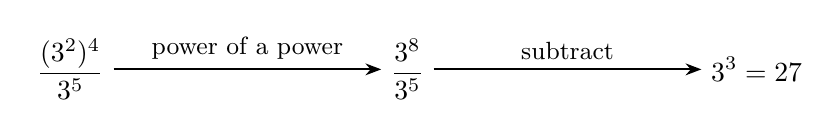
\begin{tikzpicture}[>={Stealth[length=2mm]},node distance=1.5cm and 3.4cm]
\node (s0) {$\displaystyle \dfrac{(3^{2})^{4}}{3^{5}}$};
\node (s1) [right=of s0] {$\displaystyle \dfrac{3^{8}}{3^{5}}$};
\node (s2) [right=of s1] {$\displaystyle 3^{3}=27$};
\draw[->,thick] (s0) -- (s1) node[midway,above,font=\small]{power of a power};
\draw[->,thick] (s1) -- (s2) node[midway,above,font=\small]{subtract};
\end{tikzpicture}
}
\end{center}
\small Solution flow: each arrow applies one index law.\normalsize

\medskip\hrule

\section*{Laws of Indices 46\quad\small\texttt{(a4-046)}}
\addcontentsline{toc}{section}{Laws of Indices 46 (a4-046)}
\textit{Difficulty: Foundation \quad\textbar\quad Marks: 1}

\question{Evaluate: \( 2^{-3} \)}

\textbf{Worked solution.}

\textit{Step 1: A negative exponent means take the reciprocal.}
\[\begin{gathered}
2^{-3} = \frac{1}{2^3}
\end{gathered}\]
\( a^{-n} = \frac{1}{a^n} \).

\textit{Step 2: Evaluate \( 2^3 \).}
\[\begin{gathered}
\frac{1}{8}
\end{gathered}\]
\( 2 \times 2 \times 2 = 8 \).

\begin{answerbox}
\textbf{Final answer:}\quad \(\displaystyle \frac{1}{8}\)
\end{answerbox}
\textbf{Diagram.}

\begin{center}
\resizebox{\ifdim\width>\linewidth \linewidth\else \width\fi}{!}{%
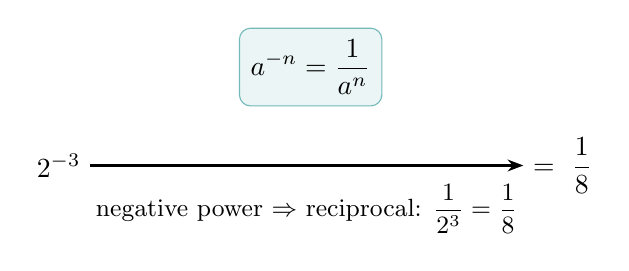
\begin{tikzpicture}[>={Stealth[length=2mm]}]
\node[draw=teal!55,rounded corners,fill=teal!8,inner sep=4pt] (rule) at (3.2,1.25) {$\displaystyle a^{-n}=\dfrac{1}{a^{n}}$};
\node (L) at (0,0) {$\displaystyle 2^{-3}$};
\node (R) at (6.4,0) {$\displaystyle =\ \dfrac{1}{8}$};
\draw[->,thick] (L) -- (R) node[midway,below=3pt,font=\small,align=center]{negative power $\Rightarrow$ reciprocal: $\dfrac{1}{2^{3}}=\dfrac18$};
\end{tikzpicture}
}
\end{center}
\small Index-law card: the boxed general rule (teal) is applied to the expression.\normalsize

\medskip\hrule

\section*{Laws of Indices 47\quad\small\texttt{(a4-047)}}
\addcontentsline{toc}{section}{Laws of Indices 47 (a4-047)}
\textit{Difficulty: Foundation \quad\textbar\quad Marks: 2}

\question{Simplify, leaving your answer as a single power of \( d \): \( d^{\frac{1}{2}} \times d^{\frac{3}{2}} \)}

\textbf{Worked solution.}

\textit{Step 1: Add the fractional exponents since the bases are the same.}
\[\begin{gathered}
d^{\frac{1}{2}+\frac{3}{2}}
\end{gathered}\]
The multiplication law says \( a^m \times a^n = a^{m+n} \).

\textit{Step 2: Simplify the sum of the exponents.}
\[\begin{gathered}
d^{\frac{4}{2}} = d^{2}
\end{gathered}\]
\( \frac{1}{2} + \frac{3}{2} = \frac{4}{2} = 2 \).

\begin{answerbox}
\textbf{Final answer:}\quad \(\displaystyle d^{2}\)
\end{answerbox}
\textbf{Diagram.}

\begin{center}
\resizebox{\ifdim\width>\linewidth \linewidth\else \width\fi}{!}{%
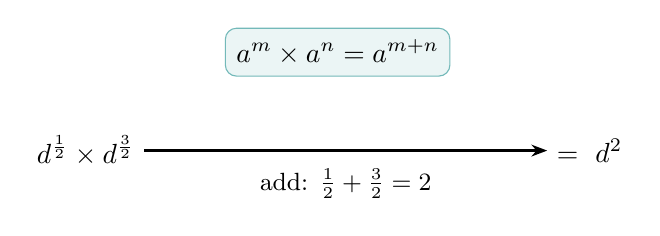
\begin{tikzpicture}[>={Stealth[length=2mm]}]
\node[draw=teal!55,rounded corners,fill=teal!8,inner sep=4pt] (rule) at (3.2,1.25) {$\displaystyle a^{m}\times a^{n}=a^{m+n}$};
\node (L) at (0,0) {$\displaystyle d^{\frac{1}{2}}\times d^{\frac{3}{2}}$};
\node (R) at (6.4,0) {$\displaystyle =\ d^{2}$};
\draw[->,thick] (L) -- (R) node[midway,below=3pt,font=\small,align=center]{add: $\tfrac12+\tfrac32=2$};
\end{tikzpicture}
}
\end{center}
\small Index-law card: the boxed general rule (teal) is applied to the expression.\normalsize

\medskip\hrule

\section*{Laws of Indices 48\quad\small\texttt{(a4-048)}}
\addcontentsline{toc}{section}{Laws of Indices 48 (a4-048)}
\textit{Difficulty: Foundation \quad\textbar\quad Marks: 2}

\question{Find the value of \( x \): \( 2^x = 16 \)}

\textbf{Worked solution.}

\textit{Step 1: Rewrite 16 as a power of 2.}
\[\begin{gathered}
16 = 2^4
\end{gathered}\]
\( 2 \times 2 \times 2 \times 2 = 16 \).

\textit{Step 2: Compare the exponents since the bases are equal.}
\[\begin{gathered}
2^x = 2^4 \implies x = 4
\end{gathered}\]
If \( a^x = a^y \) then \( x = y \).

\begin{answerbox}
\textbf{Final answer:}\quad \(\displaystyle x = 4\)
\end{answerbox}
\textbf{Diagram.}

\begin{center}
\resizebox{\ifdim\width>\linewidth \linewidth\else \width\fi}{!}{%
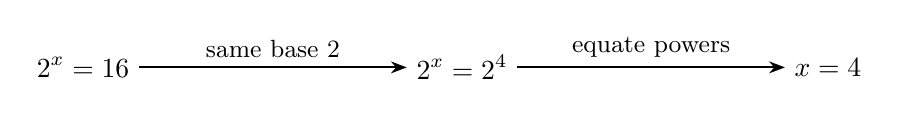
\begin{tikzpicture}[>={Stealth[length=2mm]},node distance=1.5cm and 3.4cm]
\node (s0) {$\displaystyle 2^{x}=16$};
\node (s1) [right=of s0] {$\displaystyle 2^{x}=2^{4}$};
\node (s2) [right=of s1] {$\displaystyle x=4$};
\draw[->,thick] (s0) -- (s1) node[midway,above,font=\small]{same base $2$};
\draw[->,thick] (s1) -- (s2) node[midway,above,font=\small]{equate powers};
\end{tikzpicture}
}
\end{center}
\small Solution flow: each arrow applies one index law.\normalsize

\medskip\hrule

\section*{Laws of Indices 49\quad\small\texttt{(a4-049)}}
\addcontentsline{toc}{section}{Laws of Indices 49 (a4-049)}
\textit{Difficulty: Foundation \quad\textbar\quad Marks: 2}

\question{Simplify: \( \frac{5^4 \times 5^{-2}}{5^3} \)}

\textbf{Worked solution.}

\textit{Step 1: Simplify the numerator by adding the exponents.}
\[\begin{gathered}
\frac{5^{4+(-2)}}{5^3} = \frac{5^{2}}{5^3}
\end{gathered}\]
\( 4 + (-2) = 2 \).

\textit{Step 2: Apply the division law.}
\[\begin{gathered}
5^{2-3} = 5^{-1}
\end{gathered}\]
\( 2 - 3 = -1 \).

\textit{Step 3: Evaluate.}
\[\begin{gathered}
5^{-1} = \frac{1}{5}
\end{gathered}\]
A power of \( -1 \) means the reciprocal.

\begin{answerbox}
\textbf{Final answer:}\quad \(\displaystyle \frac{1}{5}\)
\end{answerbox}
\textbf{Diagram.}

\begin{center}
\resizebox{\ifdim\width>\linewidth \linewidth\else \width\fi}{!}{%
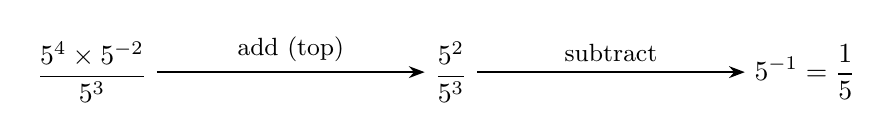
\begin{tikzpicture}[>={Stealth[length=2mm]},node distance=1.5cm and 3.4cm]
\node (s0) {$\displaystyle \dfrac{5^{4}\times 5^{-2}}{5^{3}}$};
\node (s1) [right=of s0] {$\displaystyle \dfrac{5^{2}}{5^{3}}$};
\node (s2) [right=of s1] {$\displaystyle 5^{-1}=\dfrac{1}{5}$};
\draw[->,thick] (s0) -- (s1) node[midway,above,font=\small]{add (top)};
\draw[->,thick] (s1) -- (s2) node[midway,above,font=\small]{subtract};
\end{tikzpicture}
}
\end{center}
\small Solution flow: each arrow applies one index law.\normalsize

\medskip\hrule

\section*{Laws of Indices 50\quad\small\texttt{(a4-050)}}
\addcontentsline{toc}{section}{Laws of Indices 50 (a4-050)}
\textit{Difficulty: Foundation \quad\textbar\quad Marks: 2}

\question{Evaluate: \( 8^{\frac{2}{3}} \)}

\textbf{Worked solution.}

\textit{Step 1: Split the fractional exponent: cube root first, then square.}
\[\begin{gathered}
8^{\frac{2}{3}} = \left(8^{\frac{1}{3}}\right)^2
\end{gathered}\]
The denominator 3 means take the cube root; the numerator 2 means square.

\textit{Step 2: Take the cube root of 8.}
\[\begin{gathered}
8^{\frac{1}{3}} = 2
\end{gathered}\]
\( 2 \times 2 \times 2 = 8 \).

\textit{Step 3: Square the result.}
\[\begin{gathered}
2^2 = 4
\end{gathered}\]
\( 2 \times 2 = 4 \).

\begin{answerbox}
\textbf{Final answer:}\quad \(\displaystyle 4\)
\end{answerbox}
\textbf{Diagram.}

\begin{center}
\resizebox{\ifdim\width>\linewidth \linewidth\else \width\fi}{!}{%
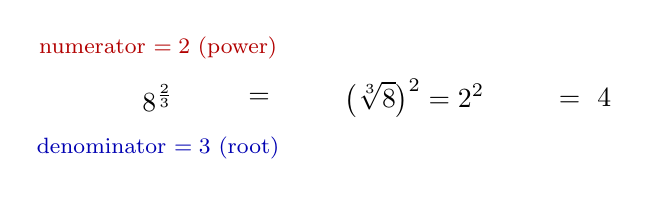
\begin{tikzpicture}[node distance=5mm and 7mm]
\node (e) {$\displaystyle 8^{\frac{2}{3}}$};
\node (eq) [right=of e] {$=$};
\node (mid) [right=of eq] {$\displaystyle \big(\sqrt[3]{8}\big)^{2}=2^{2}$};
\node (res) [right=of mid] {$\displaystyle =\ 4$};
\node[red!70!black,font=\footnotesize,above=2pt of e] {numerator $=2$ (power)};
\node[blue!70!black,font=\footnotesize,below=2pt of e] {denominator $=3$ (root)};
\end{tikzpicture}
}
\end{center}
\small Fractional index: the \emph{denominator} gives the root, the \emph{numerator} gives the power.\normalsize

\medskip\hrule

\end{document}
